\subsection{Endogenous IFIT Interaction with RSV Inclusion Bodies} \label{subsec:Endogenous IFIT Interaction with RSV Inclusion Bodies}
\subsubsection{Phenotypic Diversity of Endogenous IFIT1 Interaction with RSV IBs}
The initial exploration suggested that human IFIT1 colocalises with hRSV IBs in the A549 cell line. However, a detailed analysis of all 281 observations reveals a range of phenotypic diversities in hIFIT1 interactions with these structures. As depicted in Figure \ref{fig:Phenotypic Diversity of hIFIT1 Interactions with hRSV Inclusion Bodies in A549 Cell Line}, panel (a), approximately 30\% of interactions result in either full or partial exclusion from the structure or even diffusion through the IB and the surrounding cytosol. The next most common phenotype, occurring in approximately 18\% of observations, is inclusion inside the IB structure. Following phenotypes, each occurring at a frequency of 9\%, include colocalisation with the edge of the inclusion body joined with exclusion from the area of the IB, and an edge exclusion phenotype, where IFIT1 is present equally between the IB and the surrounding cytoplasm, except for the IB boundary, where its signal is decreased. Representative images of these phenotypes can be observed in Figure \ref{fig:Representative Images of Phenotypic Diversity of hIFIT1 Interactions with hRSV Inclusion Bodies in A549 Cell Line}. Additionally, we observed IFIT1 displaying edge exclusion with obvious spots within the IB structure. However, these phenotypes did not occur with a sufficiently high frequency to be deemed relevant during infection, as opposed to potentially being imaging artefacts. In Figure \ref{fig:Phenotypic Diversity of hIFIT1 Interactions with hRSV Inclusion Bodies in A549 Cell Line}, panel (b), the measured areas of the IBs associated with phenotypes occurring at a frequency higher than 5\% are displayed. The two most common phenotypes, exclusion and diffusion, had median IB area sizes of 5 and 4.4 \(\mu \mbox{m}^2\), values either identical or very similar to the aggregated typical IB area of all observations in the A549 cell line. Both phenotypes encompass a range of IB sizes, from sub 1 \(\mu \mbox{m}^2\) to supra 20 \(\mu \mbox{m}^2\) IB areas. On the other hand, the other observed phenotypes are more prevalent in larger inclusion bodies. In more detail, the inclusion phenotype was more prevalent in supra 3 \(\mu \mbox{m}^2\) inclusion bodies, with a typical size of 8; the colocalisation accompanied by exclusion phenotype had a median IB size of 12 \(\mu \mbox{m}^2\), although some IBs with sizes between 0.8 and 5 \(\mu \mbox{m}^2\) showed this phenotype as well; and the edge exclusion phenotype was observed in IBs with a median size of 7 \(\mu \mbox{m}^2\), although these IBs were clustered in two groups with typical values of approximately 5 and 10 \(\mu \mbox{m}^2\) respectively. Our data indicates that while in the majority of cases, IFIT1 is either excluded or diffused throughout the IB structures, regardless of the IB size and thus maturity, there is a potential interaction with more mature IBs of sizes above 5 \(\mu \mbox{m}^2\), coinciding with the IB sizes that typically have IBAGs present \cite{Rincheval2017FunctionalVirus}.

\begin{figure}
    \begin{subfigure}{0.495\textwidth}
        \caption{}
        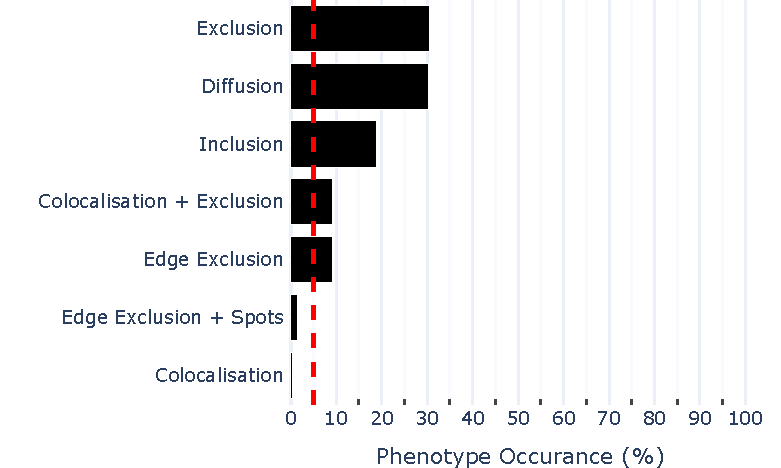
\includegraphics[width=1\linewidth]{08. Chapter 3/Figs/02. Infection/01. IFIT1/01. bar_i1_a549.pdf} 
    \end{subfigure}
    \begin{subfigure}{0.495\textwidth}
        \caption{}
        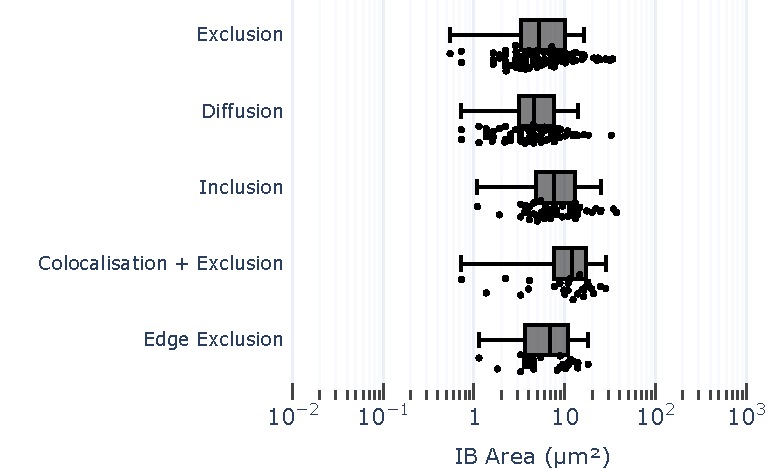
\includegraphics[width=1\linewidth]{08. Chapter 3/Figs/02. Infection/01. IFIT1/02. box_i1_a549.pdf}
    \end{subfigure}
    \caption[Phenotypic Diversity of hIFIT1 Interactions with hRSV Inclusion Bodies in A549 Cell Line.]{\textbf{Phenotypic Diversity of hIFIT1 Interactions with hRSV Inclusion Bodies in A549 Cell Line.} A549 cells were infected with human RSV at MOI 1 and fixed 24 HPI. Cells were double-labelled with anti-RSV N and anti-IFIT1 antibodies and imaged on a confocal microscope. Panel (a) shows the percentual proportions of observed phenotypes between hRSV inclusion bodies and hIFIT1 (281 observations), with the red dotted line denoting the 5\% threshold, marking phenotypes considered relevant above this limit. Panel (b) shows the IB area in \(\mu \mbox{m}^2\) per observed relevant phenotype.}
    \label{fig:Phenotypic Diversity of hIFIT1 Interactions with hRSV Inclusion Bodies in A549 Cell Line}
\end{figure}

\begin{figure}
    \centering
    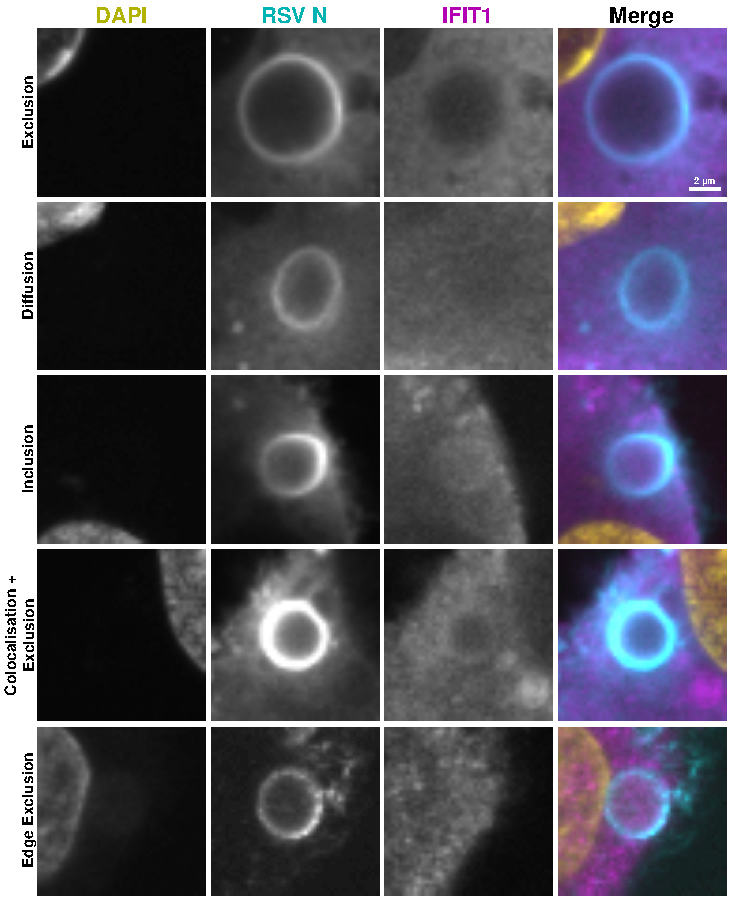
\includegraphics[width=1\linewidth]{08. Chapter 3/Figs/02. Infection/01. IFIT1/03. a549 i1.pdf}
    \caption[Representative Images of Phenotypic Diversity of hIFIT1 Interactions with hRSV Inclusion Bodies in A549 Cell Line.]{\textbf{Representative Images of Phenotypic Diversity of hIFIT1 Interactions with hRSV Inclusion Bodies in A549 Cell Line.} A549 cells were infected with hRSV at MOI 1 and fixed at 24 HPI. Cellular nuclei were stained with DAPI (yellow), and cells were double-labeled with anti-RSV N (cyan) and anti-IFIT1 (magenta) antibodies. This figure showcases representative examples of relevant phenotypes in the interaction between hIFIT1 and hRSV inclusion bodies. These phenotypes are presented in descending order based on their percentage proportions. The scale bar indicates 2 \(\mu \mbox{m}\).}
    \label{fig:Representative Images of Phenotypic Diversity of hIFIT1 Interactions with hRSV Inclusion Bodies in A549 Cell Line}
\end{figure}

To validate the previous data, we conducted experiments in the BEAS2B cell line. Figure \ref{fig:Phenotypic Diversity of hIFIT1 Interactions with hRSV Inclusion Bodies in BEAS2B Cell Line} presents the 45 observed IFIT1/IB interaction phenotypes, their occurrence (panel a), and the underlying IB sizes (panel b). Additionally, Figure \ref{fig:Representative Images of Phenotypic Diversity of hIFIT1 Interactions with hRSV Inclusion Bodies in BEAS2B Cell Line} displays representative images of phenotypes with an occurrence above 5\%. The majority of observations revealed that IFIT1 was either partially or fully excluded from the hRSV inclusion bodies, constituting approximately 85\% of the observations. About 8\% of phenotypes exhibited diffusion, and 4\% displayed colocalisation conjoined with exclusion. The size range of IBs from which IFIT1 was excluded mirrored the aggregate distribution of all IBs detected within BEAS2B cells, having an equal median size value of 3 \(\mu \mbox{m}^2\) and ranging from sub 1 \(\mu \mbox{m}^2\) to supra 10 \(\mu \mbox{m}^2\) IBs. The second most common phenotype, and the only other surpassing 5\% of total occurrence, was the diffusion phenotype, observed only in smaller IBs, with a median size of 0.5 \(\mu \mbox{m}^2\).

\begin{figure}
    \begin{subfigure}{0.495\textwidth}
        \caption{}
        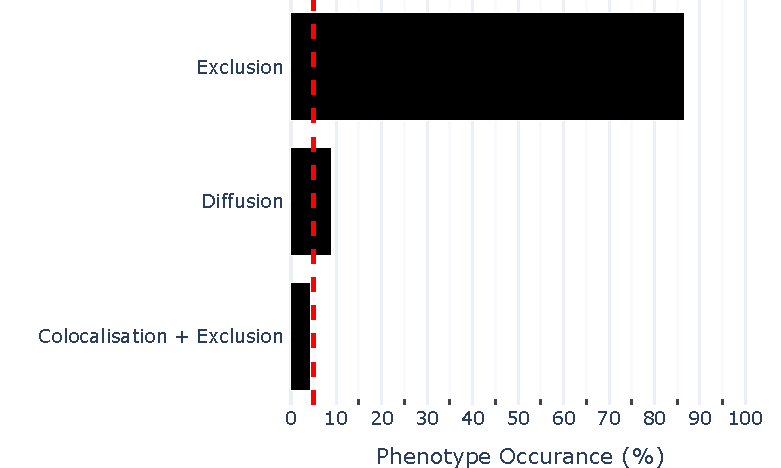
\includegraphics[width=1\linewidth]{08. Chapter 3/Figs/02. Infection/01. IFIT1/04. bar_i1_beas2b.pdf} 
    \end{subfigure}
    \begin{subfigure}{0.495\textwidth}
        \caption{}
        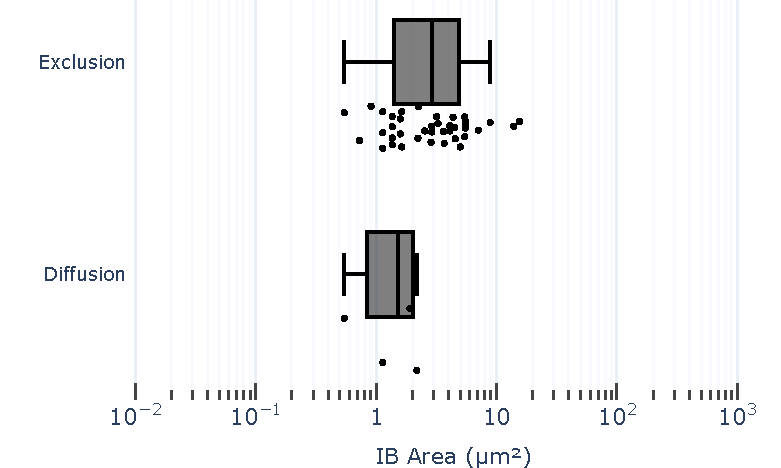
\includegraphics[width=1\linewidth]{08. Chapter 3/Figs/02. Infection/01. IFIT1/05. box_i1_beas2b.pdf}
    \end{subfigure}
    \caption[Phenotypic Diversity of hIFIT1 Interactions with hRSV Inclusion Bodies in BEAS2B Cell Line.]{\textbf{Phenotypic Diversity of hIFIT1 Interactions with hRSV Inclusion Bodies in BEAS2B Cell Line.} BEAS2B cells were infected with human RSV at MOI 1 and fixed 24 HPI. Cells were double-labelled with anti-RSV N and anti-IFIT1 antibodies and imaged on a confocal microscope. Panel (a) shows the percentual proportions of observed phenotypes between hRSV inclusion bodies and hIFIT1 (45 observations), with the red dotted line denoting the 5\% threshold, marking phenotypes considered relevant above this limit. Panel (b) shows the IB area in \(\mu \mbox{m}^2\) per observed relevant phenotype.}
    \label{fig:Phenotypic Diversity of hIFIT1 Interactions with hRSV Inclusion Bodies in BEAS2B Cell Line}
\end{figure}

\begin{figure}
    \centering
    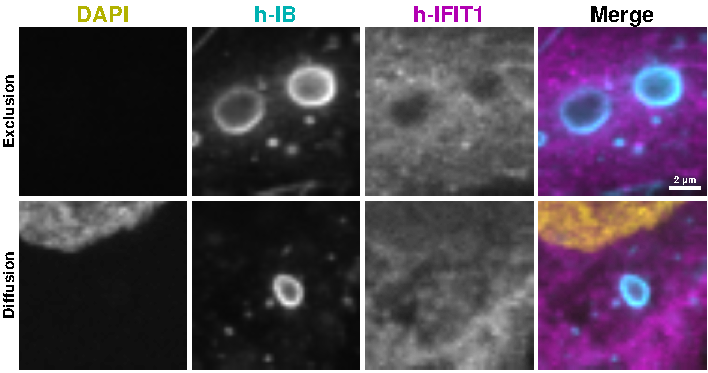
\includegraphics[width=1\linewidth]{08. Chapter 3/Figs/02. Infection/01. IFIT1/06. beas2b i1.pdf}
    \caption[Representative Images of Phenotypic Diversity of hIFIT1 Interactions with hRSV Inclusion Bodies in BEAS2B Cell Line.]{\textbf{Representative Images of Phenotypic Diversity of hIFIT1 Interactions with hRSV Inclusion Bodies in BEAS2B Cell Line.} BEAS2B cells were infected with hRSV at MOI 1 and fixed at 24 HPI. Cellular nuclei were stained with DAPI (yellow), and cells were double-labeled with anti-RSV N (cyan) and anti-IFIT1 (magenta) antibodies. This figure showcases representative examples of relevant phenotypes in the interaction between hIFIT1 and hRSV inclusion bodies. These phenotypes are presented in descending order based on their percentage proportions. The scale bar indicates 2 \(\mu \mbox{m}\).}
    \label{fig:Representative Images of Phenotypic Diversity of hIFIT1 Interactions with hRSV Inclusion Bodies in BEAS2B Cell Line}
\end{figure}

Finally, we investigated the behaviour of bovine IFIT1 during bRSV infection. Figure \ref{fig:Phenotypic Diversity of bIFIT1 Interactions with bRSV Inclusion Bodies in MDBK Cell Line} highlights the phenotypic diversity of 117 observations in detail. Similar to what was observed in A549 and BEAS2B cell lines, the most common phenotype, with around 65\% frequency, is exclusion. However, the second most common one is intra-IB inclusion (around 23\%). This is followed by the diffusion phenotype and edge exclusion, with or without the presence of possible IBAGs. Out of these, only diffusion was observed with at least 5\% frequency. Representative images of phenotypes with a frequency of occurrence above 5\% are presented in Figure \ref{fig:Representative Images of Phenotypic Diversity of bIFIT1 Interactions with bRSV Inclusion Bodies in MDBK Cell Line}. In terms of the IB size profile during each observed phenotype, the exclusion-associated IBs had a typical size of 2 \(\mu \mbox{m}^2\), with sizes ranging from sub-0.5 \(\mu \mbox{m}^2\) to supra-30 \(\mu \mbox{m}^2\), comparable with the median values of the overall distribution of the aggregate IB sizes detected in MDBK cell line. The inclusions clustered in two size ranges, predominantly to IBs with a size of around 0.9 \(\mu \mbox{m}^2\) and to IBs with sizes above 10 \(\mu \mbox{m}^2\). Lastly, we observed the diffusion phenotype to occur in IBs ranging from 0.2 \(\mu \mbox{m}^2\) to around 7 \(\mu \mbox{m}^2\), with a median value of 1.3 \(\mu \mbox{m}^2\).

Overall, our data indicate that both human and bovine IFIT1 are mainly excluded from the IBs during infection. These occurrences are present in IBs of all sizes, suggesting that this interaction phenotype is not dependent on IB maturity and complexity level. We have also observed, in all cell lines tested, IFIT1 to be diffused throughout the IB structures, which could suggest IFIT1 is able to access and thus interact with these structures. This phenotype was also observed in both small and large IBs. Most importantly, in all cell lines, we have observed IFIT1 to directly associate with IB structures, either by forming intra-IB inclusions (A549 and MDBK cell lines) or by being colocalised to the edge of the IB structure while being excluded from its inside (A549 and BEAS2B cell lines, although the frequency in BEAS2B was below 5\%). The inclusions were observed to be associated with both small and large IBs, while the colocalisation/exclusion phenotype occurred predominantly in larger, more mature IBs. This data suggests that the mechanism of action of IFIT1 inhibition of RSV replication could be mediated via IFIT1 accessing crucial RSV elements in the IBs. However, it is intriguing that we see such a diverse IFIT1/IB interaction response, and this should be investigated further.

\begin{figure}
    \begin{subfigure}{0.495\textwidth}
        \caption{}
        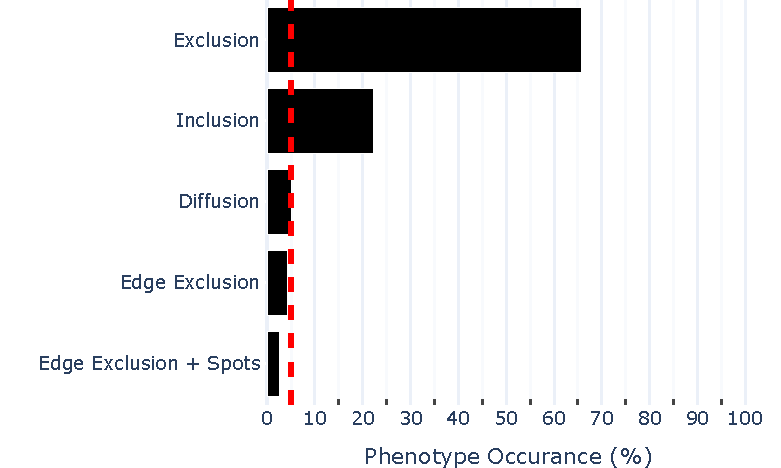
\includegraphics[width=1\linewidth]{08. Chapter 3/Figs/02. Infection/01. IFIT1/07. bar_i1_mdbk.pdf} 
    \end{subfigure}
    \begin{subfigure}{0.495\textwidth}
        \caption{}
        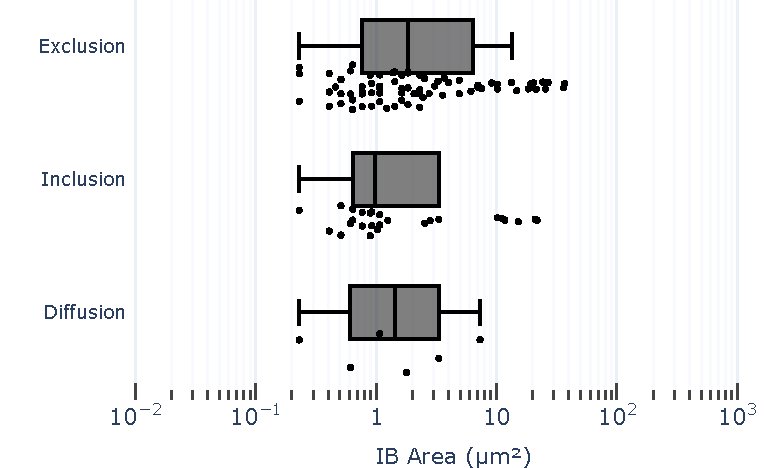
\includegraphics[width=1\linewidth]{08. Chapter 3/Figs/02. Infection/01. IFIT1/08. box_i1_mdbk.pdf}
    \end{subfigure}
    \caption[Phenotypic Diversity of bIFIT1 Interactions with bRSV Inclusion Bodies in MDBK Cell Line.]{\textbf{Phenotypic Diversity of bIFIT1 Interactions with bRSV Inclusion Bodies in MDBK Cell Line.} MDBK cells were infected with bovine RSV at MOI 1 and fixed 24 HPI. Cells were double-labelled with anti-RSV N and anti-IFIT1 antibodies and imaged on a confocal microscope. Panel (a) shows the percentual proportions of observed phenotypes between bRSV inclusion bodies and bIFIT1 (117 observations), with the red dotted line denoting the 5\% threshold, marking phenotypes considered relevant above this limit. Panel (b) shows the IB area in \(\mu \mbox{m}^2\) per observed relevant phenotype.}
    \label{fig:Phenotypic Diversity of bIFIT1 Interactions with bRSV Inclusion Bodies in MDBK Cell Line}
\end{figure}

\begin{figure}
    \centering
    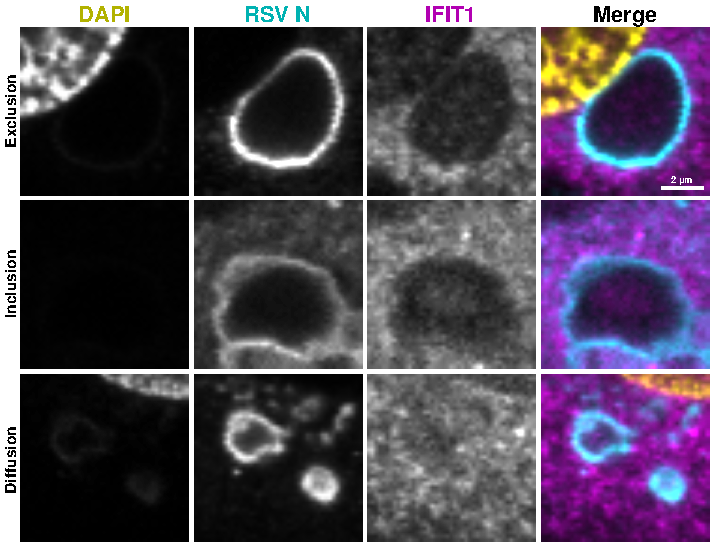
\includegraphics[width=1\linewidth]{08. Chapter 3/Figs/02. Infection/01. IFIT1/09. mdbk i1.pdf}
    \caption[Representative Images of Phenotypic Diversity of bIFIT1 Interactions with bRSV Inclusion Bodies in MDBK Cell Line.]{\textbf{Representative Images of Phenotypic Diversity of bIFIT1 Interactions with bRSV Inclusion Bodies in MDBK Cell Line.} MDBK cells were infected with bRSV at MOI 1 and fixed at 24 HPI. Cellular nuclei were stained with DAPI (yellow), and cells were double-labeled with anti-RSV N (cyan) and anti-IFIT1 (magenta) antibodies. This figure showcases representative examples of relevant phenotypes in the interaction between bIFIT1 and bRSV inclusion bodies. These phenotypes are presented in descending order based on their percentage proportions. The scale bar indicates 2 \(\mu \mbox{m}\).}
    \label{fig:Representative Images of Phenotypic Diversity of bIFIT1 Interactions with bRSV Inclusion Bodies in MDBK Cell Line}
\end{figure}

\subsubsection{Phenotypic Diversity of Endogenous IFIT2 Interaction with RSV IBs}
As described in Section \ref{subsec:IFIT Subcellular Localisation During Interferon Induction and RSV Infection}, we utilised two antibodies against IFIT2 protein, which yielded differential results with regards to both subcellular localisation and the interaction phenotype with the RSV IBs. IFIT2(A) antibody showed IFIT2 to form intra-IB inclusions in the A549 cell line, while it showed IFIT2 to colocalise with the bRSV IB boundary, while being excluded from this structure. On the other hand, IFIT2(B) antibody showed the exclusion of both human and bovine IFIT2 from the IB structures. We examined these interactions in more detail below. The results of the phenotypic diversity of the 340 interactions of IFIT2 proteins in the A549 cell line with hRSV IBs, as detected by the IFIT2(A) antibody, can be seen in Figure \ref{fig:Phenotypic Diversity of hIFIT2 Interactions with hRSV Inclusion Bodies, Detected by IFIT2(A) Antibody in A549 Cell Line}. The examples of the phenotypic interactions are shown in Figure \ref{fig:Representative Images of Phenotypic Diversity of hIFIT2 Interactions with hRSV Inclusion Bodies, Detected by IFIT2(A) Antibody in A549 Cell Line}. We can see that the most common phenotype, occurring with a frequency of 69\%, is intra-IB inclusion. This aligns with our observations from Section \ref{subsec:IFIT Subcellular Localisation During Interferon Induction and RSV Infection} (Figure \ref{fig:Alterations in the Subcellular Localisation of Human IFITs in A549 Cells Exposed to hIFNa or hRSV}), however, we see additional interactions to occur as well. Colocalisation accompanied by exclusion occurs in 30\% of observations, while an exclusion phenotype occurs in 1\% of observations. In terms of the measured areas of the IBs in which the differential interaction phenotypes occur with at least 5\% frequency, we can see that the inclusion and colocalisation accompanied by IB exclusion phenotypes clustered into two almost exclusive groups. The former had a median area of 2.1 \(\mu \mbox{m}^2\), which was lower than the median area of all A549 IB observations (which had a typical value of 5 \(\mu \mbox{m}^2\)), while the latter occurred in larger IBs, with a median size of 9 \(\mu \mbox{m}^2\). It should be noted that there is an overlap in terms of the sizes of IBs with either phenotype; however, this data suggests IFIT2 forming predominantly inclusions in immature IBs with its interaction shifting to IB boundary colocalisation with accompanied IB exclusion in the more mature IBs.

\begin{figure}
    \begin{subfigure}{0.495\textwidth}
        \caption{}
        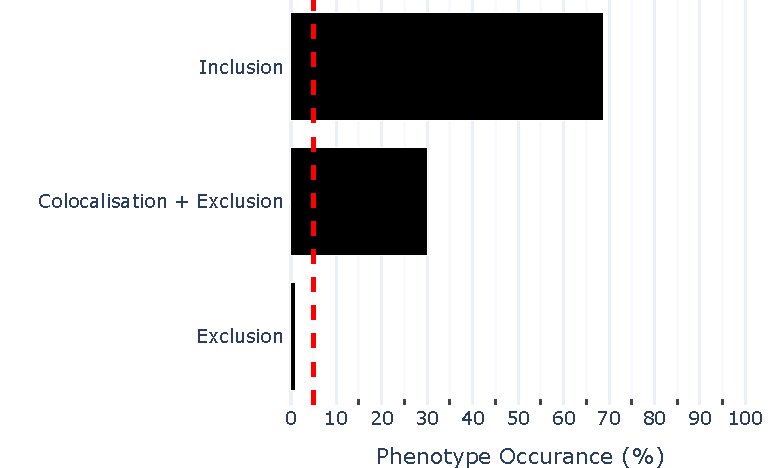
\includegraphics[width=1\linewidth]{08. Chapter 3/Figs/02. Infection/02. IFIT2/01. IFIT2A/01. bar_i2a_a549.pdf}
    \end{subfigure}
    \begin{subfigure}{0.495\textwidth}
        \caption{}
        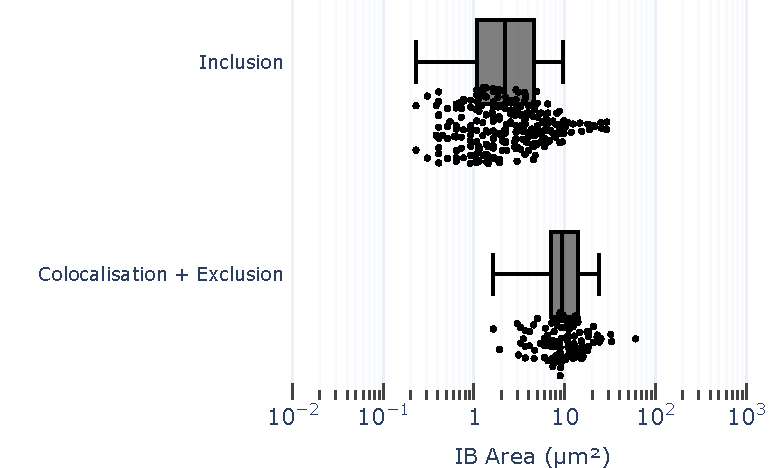
\includegraphics[width=1\linewidth]{08. Chapter 3/Figs/02. Infection/02. IFIT2/01. IFIT2A/02. box_i2a_a549.pdf}
    \end{subfigure}
    \caption[Phenotypic Diversity of hIFIT2 Interactions with hRSV Inclusion Bodies, Detected by IFIT2(A) Antibody in A549 Cell Line.]{\textbf{Phenotypic Diversity of hIFIT2 Interactions with hRSV Inclusion Bodies, Detected by IFIT2(A) Antibody in A549 Cell Line.} A549 cells were infected with human RSV at MOI 1 and fixed 24 HPI. Cells were labelled with anti-RSV N and anti-IFIT2(A) antibodies and imaged on a confocal microscope. Panel (a) shows percentual proportions of observed phenotypes between hRSV inclusion bodies and hIFIT2, detected by IFIT2(A) antibody (340 observations), with the red dotted line denoting the 5\% threshold, marking phenotypes considered relevant above this limit. Panel (b) shows the IB area in \(\mu \mbox{m}^2\) per observed relevant phenotype.}
    \label{fig:Phenotypic Diversity of hIFIT2 Interactions with hRSV Inclusion Bodies, Detected by IFIT2(A) Antibody in A549 Cell Line}
\end{figure}

\begin{figure}
    \centering
    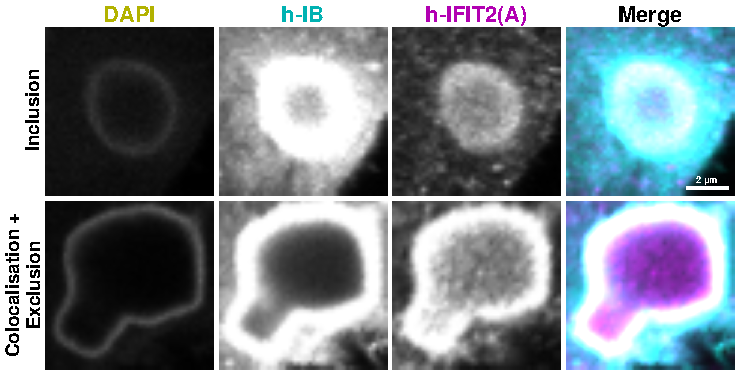
\includegraphics[width=1\linewidth]{08. Chapter 3/Figs/02. Infection/02. IFIT2/01. IFIT2A/03. i2a-a549.pdf}
    \caption[Representative Images of Phenotypic Diversity of hIFIT2 Interactions with hRSV Inclusion Bodies, Detected by IFIT2(A) Antibody in A549 Cell Line.]{\textbf{Representative Images of Phenotypic Diversity of hIFIT2 Interactions with hRSV Inclusion Bodies, Detected by IFIT2(A) Antibody in A549 Cell Line.} A549 cells were infected with hRSV at MOI 1 and fixed at 24 HPI. Cellular nuclei were stained with DAPI (yellow), and cells were double-labeled with anti-RSV N (cyan) and anti-IFIT2(A) (magenta) antibodies. This figure showcases representative examples of relevant phenotypes in the interaction between hIFIT2, detected by IFIT2(A) antibody, and hRSV inclusion bodies. These phenotypes are presented in descending order based on their percentage proportions. The scale bar indicates 2 \(\mu \mbox{m}\).}
    \label{fig:Representative Images of Phenotypic Diversity of hIFIT2 Interactions with hRSV Inclusion Bodies, Detected by IFIT2(A) Antibody in A549 Cell Line}
\end{figure}

For IFIT2 interaction phenotypes with hRSV IBs, as detected by the IFIT2(B) antibody in the A549 cell line, we observe it to conform to our previous observations from Section \ref{subsec:IFIT Subcellular Localisation During Interferon Induction and RSV Infection} (Figure \ref{fig:Alterations in the Subcellular Localisation of Human IFITs in A549 Cells Exposed to hIFNa or hRSV} and Figure \ref{fig:Modulations in the Subcellular Localisation of Bovine IFITs in MDBK Cells Exposed to bIFNa or bRSV}). The underlying phenotype frequency data of these 230 observations, along with the measured IB sizes, can be seen in Figure \ref{fig:Phenotypic Diversity of hIFIT2 Interactions with hRSV Inclusion Bodies, Detected by IFIT2(B) Antibody in A549 Cell Line}, while the representative images of the major occurring phenotype can be seen in Figure \ref{fig:Representative Images of Phenotypic Diversity of hIFIT2 Interactions with hRSV Inclusion Bodies, Detected by IFIT2(B) Antibody in A549 Cell Line}. We can see that in 97\% of IB occurrences, IFIT2 was found to be excluded from the structure. 3\% of the observations showed IFIT2 to be diffused through both the cytoplasm and the IB structure. In terms of the size profile of the exclusion-associated IBs, they have a minimal size of 4 \(\mu \mbox{m}^2\), median size of 5 \(\mu \mbox{m}^2\), and a maximal observed size of supra 30 \(\mu \mbox{m}^2\). This distribution is nearly identical to the aggregate distribution of all IBs detected in A549 in this study (Section \ref{subsec:IFIT Subcellular Localisation During Interferon Induction and RSV Infection}, Figure \ref{fig:The Distributions of IB Areas Observed Per Cell Line}), which allows us to confirm that IFIT2, as detected by the IFIT2(B) antibody in A549 cell line, is excluded from these structures regardless of the IB size and thus maturity, and these results are not a result of observational bias.

\begin{figure}
    \begin{subfigure}{0.495\textwidth}
        \caption{}
        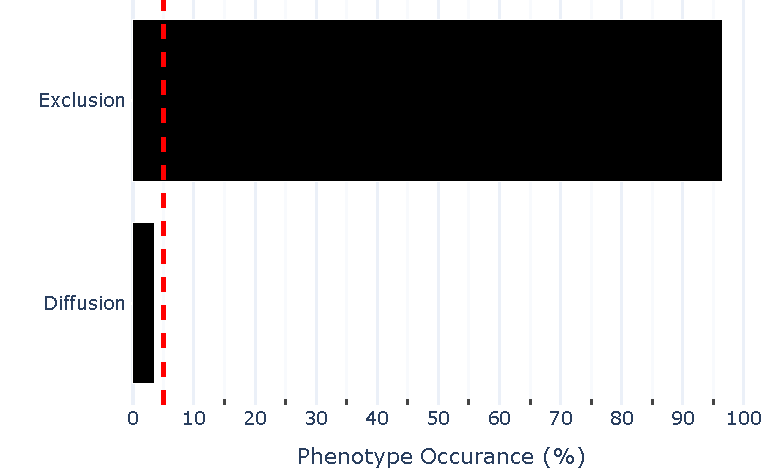
\includegraphics[width=1\linewidth]{08. Chapter 3/Figs/02. Infection/02. IFIT2/02. IFIT2B/01. bar_i2b_a549.pdf}
    \end{subfigure}
    \begin{subfigure}{0.495\textwidth}
        \caption{}
        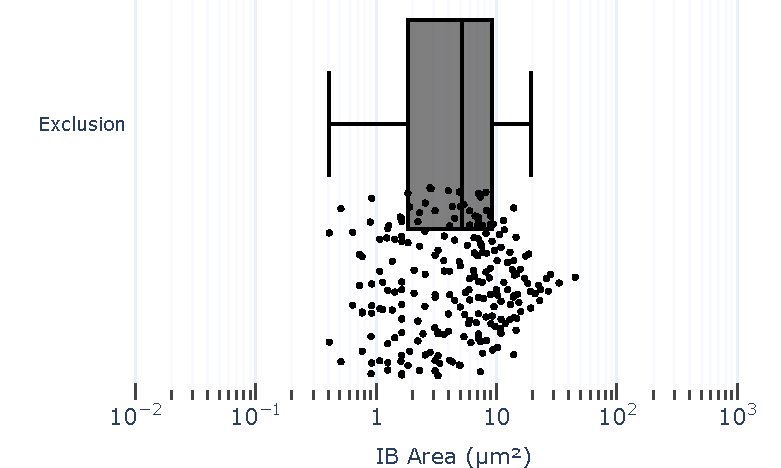
\includegraphics[width=1\linewidth]{08. Chapter 3/Figs/02. Infection/02. IFIT2/02. IFIT2B/02. box_i2b_a549.pdf}
    \end{subfigure}
    \caption[Phenotypic Diversity of hIFIT2 Interactions with hRSV Inclusion Bodies, Detected by IFIT2(B) Antibody in A549 Cell Line.]{\textbf{Phenotypic Diversity of hIFIT2 Interactions with hRSV Inclusion Bodies, Detected by IFIT2(B) Antibody in A549 Cell Line.} A549 cells were infected with human RSV at MOI 1 and fixed 24 HPI. Cells were labeled with anti-RSV N and anti-IFIT2(B) antibodies and imaged on confocal microscope. Panel (a) shows percentual proportions of observed phenotypes between hRSV inclusion bodies and hIFIT2, detected by IFIT2(B) antibody (230 observations), with the red dotted line denoting the 5\% threshold, marking phenotypes considered relevant above this limit. Panel (b) shows the IB area in \(\mu \mbox{m}^2\) per observed relevant phenotype.}
    \label{fig:Phenotypic Diversity of hIFIT2 Interactions with hRSV Inclusion Bodies, Detected by IFIT2(B) Antibody in A549 Cell Line}
\end{figure}

\begin{figure}
    \centering
    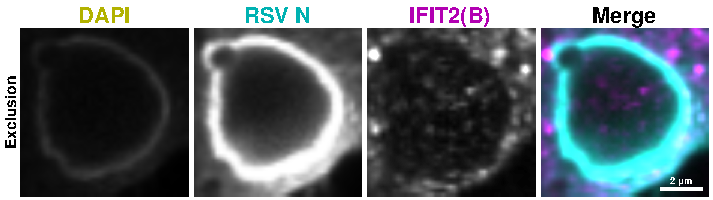
\includegraphics[width=1\linewidth]{08. Chapter 3/Figs/02. Infection/02. IFIT2/02. IFIT2B/03. i2b-a549.pdf} 
    \caption[Representative Images of Phenotypic Diversity of hIFIT2 Interactions with hRSV Inclusion Bodies, Detected by IFIT2(B) Antibody in A549 Cell Line.]{\textbf{Representative Images of Phenotypic Diversity of hIFIT2 Interactions with hRSV Inclusion Bodies, Detected by IFIT2(B) Antibody in A549 Cell Line.} A549 cells were infected with hRSV at MOI 1 and fixed at 24 HPI. Cellular nuclei were stained with DAPI (yellow), and cells were double-labelled with anti-RSV N (cyan) and anti-IFIT2(B) (magenta) antibodies. This figure showcases representative examples of relevant phenotypes in the interaction between hIFIT2, detected by IFIT2(B) antibody, and hRSV inclusion bodies. These phenotypes are presented in descending order based on their percentage proportions. The scale bar indicates 2 \(\mu \mbox{m}\).}
    \label{fig:Representative Images of Phenotypic Diversity of hIFIT2 Interactions with hRSV Inclusion Bodies, Detected by IFIT2(B) Antibody in A549 Cell Line}
\end{figure}

Seeing that the IFIT2(A) antibody showed results of human IFIT2 localisations not observed previously in our study, while the IFIT2(B) antibody showed results that were consistent with our previous data (both referring to the data from Section \ref{subsec:IFIT Subcellular Localisation During Interferon Induction and RSV Infection}, Figure \ref{fig:Alterations in the Subcellular Localisation of Human IFITs in A549 Cells Exposed to hIFNa or hRSV}), we decided to validate the IFIT2(A) results using the BEAS2B cell line infected with hRSV at MOI 1. Samples were fixed 24 HPI. The phenotypic diversity data can be seen in Figure \ref{fig:Phenotypic Diversity of hIFIT2 Interactions with hRSV Inclusion Bodies, Detected by IFIT2(A) Antibody in BEAS2B Cell Line}, while the representative images of these phenotypes are shown in Figure \ref{fig:Representative Images of Phenotypic Diversity of hIFIT2 Interactions with hRSV Inclusion Bodies, Detected by IFIT2(A) Antibody in BEAS2B Cell Line}. It is to be noted that we had only a small number of observations for this sample (17 observations). Regardless, the results are fairly consistent with the ones from the A549 cell line. We see that the most commonly observed phenotype is colocalisation accompanied by IB exclusion with a frequency of 59\%, followed by the inclusion phenotype (35\%), and lastly the diffusion phenotype (6\% of observations). Compared to the results from the A549 cell line, the two top phenotypes are reversed, although this could be due to a bias caused by a low sample size. The colocalisation and exclusion phenotype occurred in IBs with their sizes ranging from sub 1 \(\mu \mbox{m}^2\) to 8 \(\mu \mbox{m}^2\), with the median size of 3 \(\mu \mbox{m}^2\). This is also the median size of IBs from the aggregate of all observations, suggesting this phenotype distribution coincides with the overall distribution of IB sizes in BEAS2B cell line 24 HPI. The inclusion and diffusion phenotypes occur in smaller IBs with the median sizes of 1.1 \(\mu \mbox{m}^2\) and 1.3 \(\mu \mbox{m}^2\) respectively, with the inclusion phenotype-associated IBs sizes ranging from sub 1 \(\mu \mbox{m}^2\) to 5 \(\mu \mbox{m}^2\).

\begin{figure}
    \begin{subfigure}{0.495\textwidth}
        \caption{}
        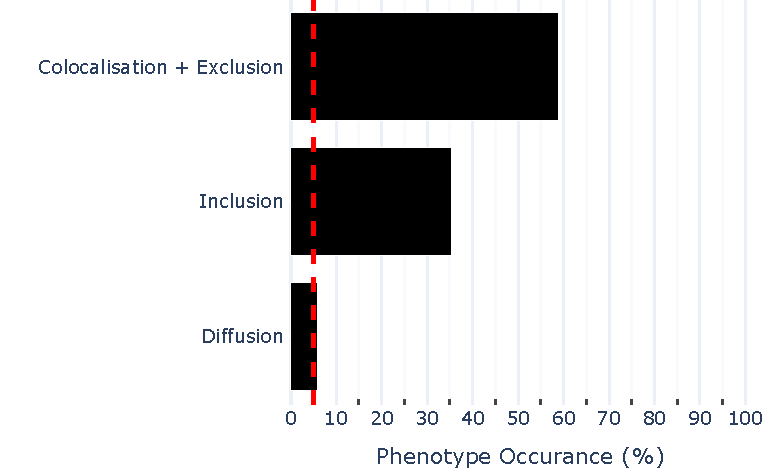
\includegraphics[width=1\linewidth]{08. Chapter 3/Figs/02. Infection/02. IFIT2/01. IFIT2A/10. bar_i2a_beas2b.pdf} 
    \end{subfigure}
    \begin{subfigure}{0.495\textwidth}
        \caption{}
        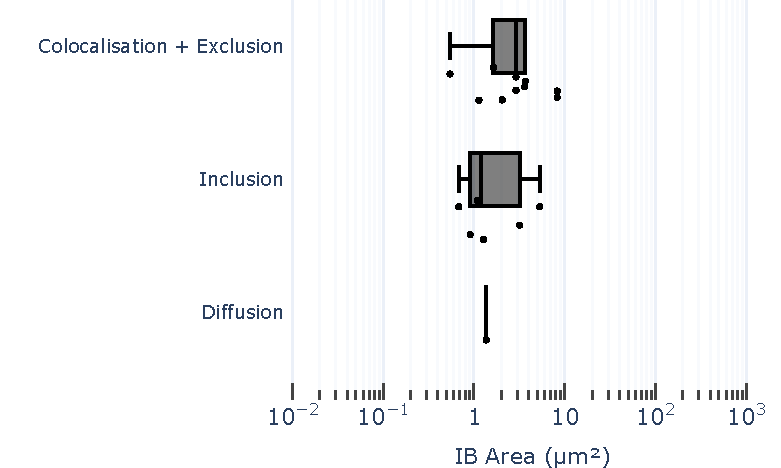
\includegraphics[width=1\linewidth]{08. Chapter 3/Figs/02. Infection/02. IFIT2/01. IFIT2A/11. box_i2a_beas2b.pdf}
    \end{subfigure}
    \caption[Phenotypic Diversity of hIFIT2 Interactions with hRSV Inclusion Bodies, Detected by IFIT2(A) Antibody in BEAS2B Cell Line.]{\textbf{Phenotypic Diversity of hIFIT2 Interactions with hRSV Inclusion Bodies, Detected by IFIT2(A) Antibody in BEAS2B Cell Line.} BEAS2B cells were infected with human RSV at MOI 1 and fixed 24 HPI. Cells were labeled with anti-RSV N and anti-IFIT2(A) antibodies and imaged on confocal microscope. Panel (a) shows percentual proportions of observed phenotypes between hRSV inclusion bodies and hIFIT2, detected by IFIT2(A) antibody (17 observations), with the red dotted line denoting the 5\% threshold, marking phenotypes considered relevant above this limit. Panel (b) shows the IB area in \(\mu \mbox{m}^2\) per observed relevant phenotype.}
    \label{fig:Phenotypic Diversity of hIFIT2 Interactions with hRSV Inclusion Bodies, Detected by IFIT2(A) Antibody in BEAS2B Cell Line}
\end{figure}

\begin{figure}
    \centering
    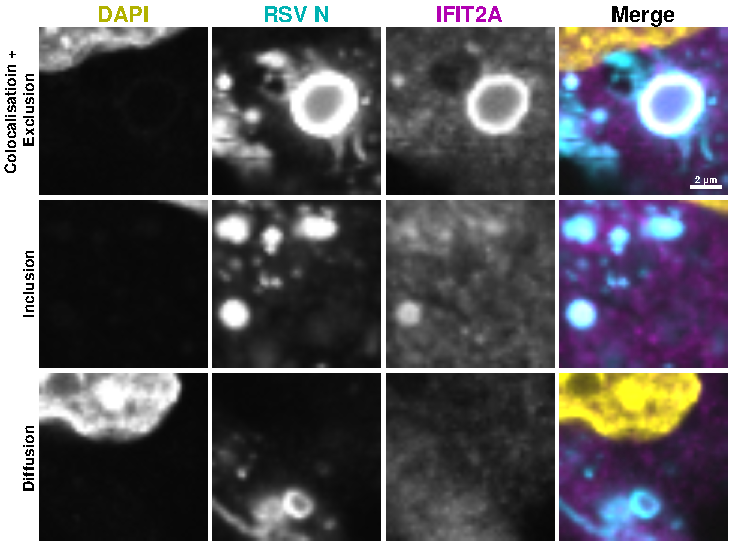
\includegraphics[width=1\linewidth]{08. Chapter 3/Figs/02. Infection/02. IFIT2/01. IFIT2A/12. i2a beas2b.pdf} 
    \caption[Representative Images of Phenotypic Diversity of hIFIT2 Interactions with hRSV Inclusion Bodies, Detected by IFIT2(A) Antibody in BEAS2B Cell Line.]{\textbf{Representative Images of Phenotypic Diversity of hIFIT2 Interactions with hRSV Inclusion Bodies, Detected by IFIT2(A) Antibody in BEAS2B Cell Line.} BEAS2B cells were infected with hRSV at MOI 1 and fixed at 24 HPI. Cellular nuclei were stained with DAPI (yellow), and cells were double-labelled with anti-RSV N (cyan) and anti-IFIT2(A) (magenta) antibodies. This figure showcases representative examples of relevant phenotypes in the interaction between hIFIT2, detected by IFIT2(A) antibody, and hRSV inclusion bodies. These phenotypes are presented in descending order based on their percentage proportions. The scale bar indicates 2 \(\mu \mbox{m}\).}
    \label{fig:Representative Images of Phenotypic Diversity of hIFIT2 Interactions with hRSV Inclusion Bodies, Detected by IFIT2(A) Antibody in BEAS2B Cell Line}
\end{figure}

Analyzing the phenotypic diversity in 162 observations of bovine IFIT2 interaction with bRSV IBs in MDBK cell line, as detected by the IFIT2(A) antibody, we see data consistent with observations in A549 and BEAS2B cell lines. Although in the initial analysis, we observed IFIT2 to colocalise with the bRSV IB boundary, we again see two distinct phenotypes occurring, namely the inclusion phenotype (64\% of occurrences) and the colocalisation accompanied by exclusion phenotype (36\% of occurrences). The IBs associated with these interaction phenotypes had median areas of 0.9 \(\mu \mbox{m}^2\) and 9 \(\mu \mbox{m}^2\) respectively. These data can be seen in Figure \ref{fig:Phenotypic Diversity of bIFIT2 Interactions with bRSV Inclusion Bodies, Detected by IFIT2(A) Antibody in MDBK Cell Line}, with the representative images of these phenotypes shown in Figure \ref{fig:Representative Images of Phenotypic Diversity of bIFIT2 Interactions with bRSV Inclusion Bodies, Detected by IFIT2(A) Antibody in MDBK Cell Line}. Similar to what was observed in A549 (Figure \ref{fig:Phenotypic Diversity of hIFIT2 Interactions with hRSV Inclusion Bodies, Detected by IFIT2(A) Antibody in A549 Cell Line}), the two observed interaction phenotypes aggregate in two inner-overlapping clusters, which suggests these phenotypes are associated with IBs of differential maturity, and the inner overlap is a transition phase from one phenotype/maturity stage to another.

\begin{figure}
    \begin{subfigure}{0.495\textwidth}
        \caption{}
        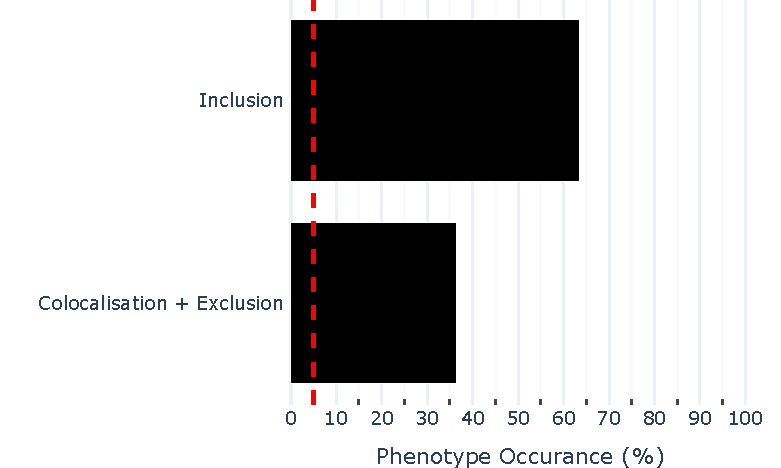
\includegraphics[width=1\linewidth]{08. Chapter 3/Figs/02. Infection/02. IFIT2/01. IFIT2A/13. bar_i2a_mdbk.pdf} 
    \end{subfigure}
    \begin{subfigure}{0.495\textwidth}
        \caption{}
        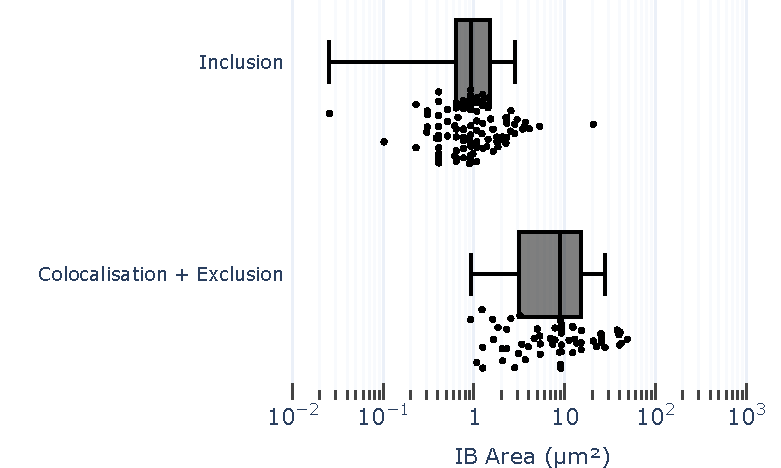
\includegraphics[width=1\linewidth]{08. Chapter 3/Figs/02. Infection/02. IFIT2/01. IFIT2A/14. box_i2a_mdbk.pdf}
    \end{subfigure}
    \caption[Phenotypic Diversity of bIFIT2 Interactions with bRSV Inclusion Bodies, Detected by IFIT2(A) Antibody in MDBK Cell Line.]{\textbf{Phenotypic Diversity of bIFIT2 Interactions with bRSV Inclusion Bodies, Detected by IFIT2(A) Antibody in MDBK Cell Line.} MDBK cells were infected with bovine RSV at MOI 1 and fixed 24 HPI. Cells were labelled with anti-RSV N and anti-IFIT2(A) antibodies and imaged on a confocal microscope. Panel (a) shows percentual proportions of observed phenotypes between bRSV inclusion bodies and bIFIT2, detected by IFIT2(A) antibody (162 observations), with the red dotted line denoting the 5\% threshold, marking phenotypes considered relevant above this limit. Panel (b) shows the IB area in \(\mu \mbox{m}^2\) per observed relevant phenotype.}
    \label{fig:Phenotypic Diversity of bIFIT2 Interactions with bRSV Inclusion Bodies, Detected by IFIT2(A) Antibody in MDBK Cell Line}
\end{figure}

\begin{figure}
    \centering
    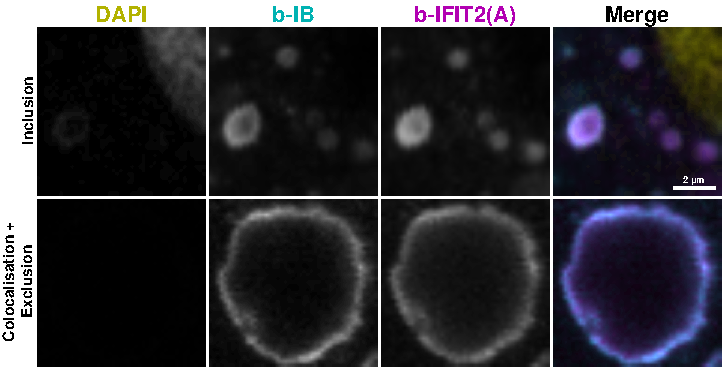
\includegraphics[width=1\linewidth]{08. Chapter 3/Figs/02. Infection/02. IFIT2/01. IFIT2A/15. i2a mdbk brsv.pdf} 
    \caption[Representative Images of Phenotypic Diversity of bIFIT2 Interactions with bRSV Inclusion Bodies, Detected by IFIT2(A) Antibody in MDBK Cell Line.]{\textbf{Representative Images of Phenotypic Diversity of bIFIT2 Interactions with bRSV Inclusion Bodies, Detected by IFIT2(A) Antibody in MDBK Cell Line.} MDBK cells were infected with bRSV at MOI 1 and fixed at 24 HPI. Cellular nuclei were stained with DAPI (yellow), and cells were double-labelled with anti-RSV N (cyan) and anti-IFIT2(A) (magenta) antibodies. This figure showcases representative examples of relevant phenotypes in the interaction between bIFIT2, detected by IFIT2(A) antibody, and bRSV inclusion bodies. These phenotypes are presented in descending order based on their percentage proportions. The scale bar indicates 2 \(\mu \mbox{m}\).}
    \label{fig:Representative Images of Phenotypic Diversity of bIFIT2 Interactions with bRSV Inclusion Bodies, Detected by IFIT2(A) Antibody in MDBK Cell Line}
\end{figure}

Lastly, we assayed the phenotypic diversity of 66 observations of bovine IFIT2 with bRSV IBs in MDBK cell line as detected by IFIT2(B) antibody (Figure \ref{fig:Phenotypic Diversity of hIFIT2 Interactions with bRSV Inclusion Bodies, Detected by IFIT2(B) Antibody in MDBK Cell Line}), with the representative images shown in Figure \ref{fig:Representative Images of Phenotypic Diversity of hIFIT2 Interactions with bRSV Inclusion Bodies, Detected by IFIT2(B) Antibody in MDBK Cell Line}. We observed 4 interaction phenotypes to occur, namely exclusion (71\% occurrence), IB edge exclusion with intra IB spots (21\% occurrence), diffusion (6\% occurrence), and edge exclusion phenotype without intra IB spots, which occurred in only 1\% of observations. When looking at the size profile of the IBs associated with the commonly occurring phenotypes (>5\%), we can see a separation by IB area. The exclusion interaction phenotype happened in IBs with the median size of 2.2 \(\mu \mbox{m}^2\), a value almost equivalent to the median aggregate value observed in MDBK cell line (2 \(\mu \mbox{m}^2\)), suggesting this phenotype is a good proxy for the whole IB population-level interaction. The second most common phenotype, edge exclusion with the presence of spots, occurred in IBs ranging from 0.5 \(\mu \mbox{m}^2\) to supra 20 \(\mu \mbox{m}^2\), with the typical value of 7 \(\mu \mbox{m}^2\). The majority of the IBs observed to associate with this phenotype were larger than 4 \(\mu \mbox{m}^2\), a size boundary reported to distinguish IBAG-containing IBs, although it is to be noted that a considerable proportion of the IBs were smaller than this value, and thus probably IBAG-less. What this means is the intra IB IFIT2 structures we observed seem not to always be IGAGs, if ever. Lastly, the phenotypic interaction where IFIT2 was seen to be equally diffused throughout the cytoplasm and the IB structure occurred in large IBs with the median size of 15 \(\mu \mbox{m}^2\).

The obtained IFIT2/IB interaction results are remarkably consistent within each antibody used. The IFIT2(A) antibody consistently detected IFIT2 interacting with the IB structures in a bimodal fashion. IFIT2 was observed to form intra-IB inclusions in small and medium-sized IBs and to colocalise with the edge of medium and large IBs, while being excluded from their interior. This data hints at a gradual change in the IFIT2/IB interaction as a function of IB maturation. It appears that as the IBs are formed, IFIT2 is recruited to these structures, but as their size and internal complexity increase, it preferentially condenses at the IB boundary. On the other hand, IFIT2(B)-stained IFIT2 consistently demonstrated exclusion from the IB structures, regardless of the cell line and RSV strain used. These data likely indicate the presence of two antigenically distinct populations of IFIT2 in both human and bovine cells, which differentially interact with the IB structures — a hypothesis that will be further explored in Chapter \ref{ch:Investigating the Nature of IFIT and IB Interactions}.

\begin{figure}
    \begin{subfigure}{0.495\textwidth}
        \caption{}
        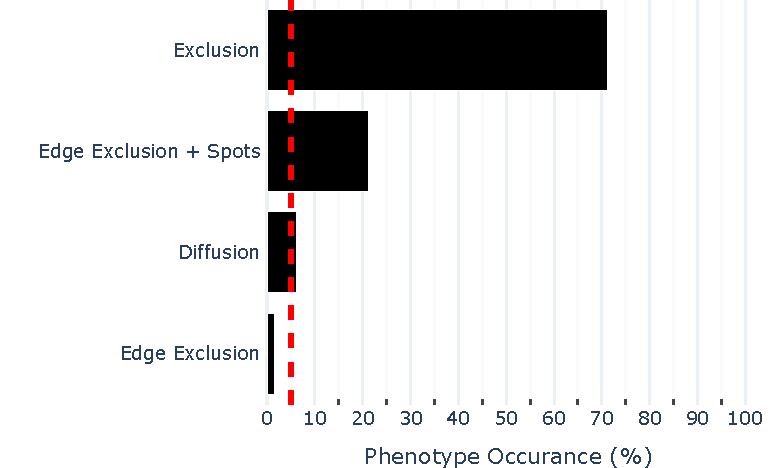
\includegraphics[width=1\linewidth]{08. Chapter 3/Figs/02. Infection/02. IFIT2/02. IFIT2B/10. bar_i2b_mdbk.pdf} 
    \end{subfigure}
    \begin{subfigure}{0.495\textwidth}
        \caption{}
        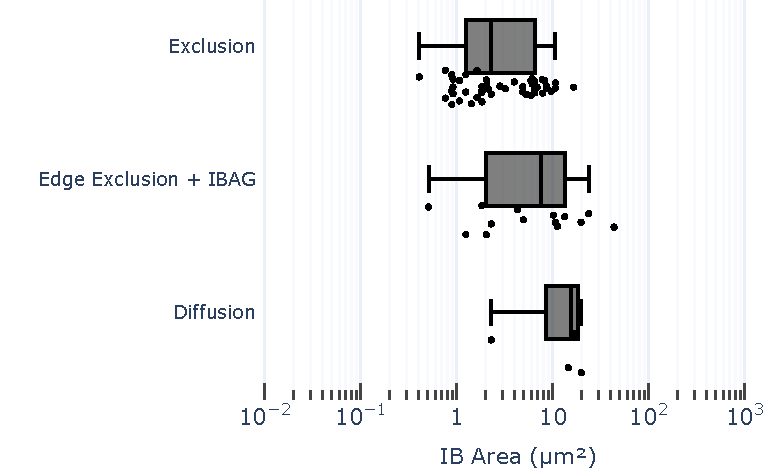
\includegraphics[width=1\linewidth]{08. Chapter 3/Figs/02. Infection/02. IFIT2/02. IFIT2B/11. box_i2b_mdbk.pdf}
    \end{subfigure}
    \caption[Phenotypic Diversity of hIFIT2 Interactions with bRSV Inclusion Bodies, Detected by IFIT2(B) Antibody in MDBK Cell Line.]{\textbf{Phenotypic Diversity of hIFIT2 Interactions with bRSV Inclusion Bodies, Detected by IFIT2(B) Antibody in MDBK Cell Line.} MDBK cells were infected with bovine RSV at MOI 1 and fixed 24 HPI. Cells were labeled with anti-RSV N and anti-IFIT2(B) antibodies and imaged on confocal microscope. Panel (a) shows percentual proportions of observed phenotypes between bRSV inclusion bodies and bIFIT2, detected by IFIT2(B) antibody (66 observations), with the red dotted line denoting the 5\% threshold, marking phenotypes considered relevant above this limit. Panel (b) shows the IB area in \(\mu \mbox{m}^2\) per observed relevant phenotype.}
    \label{fig:Phenotypic Diversity of hIFIT2 Interactions with bRSV Inclusion Bodies, Detected by IFIT2(B) Antibody in MDBK Cell Line}
\end{figure}

\begin{figure}
    \centering
    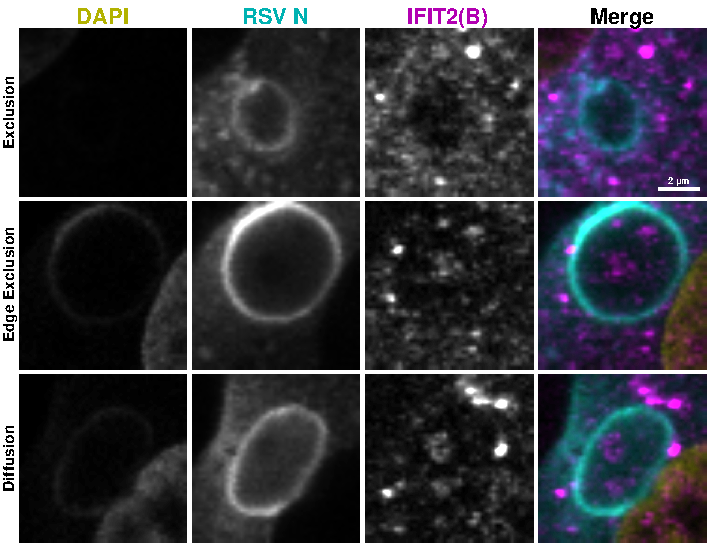
\includegraphics[width=1\linewidth]{08. Chapter 3/Figs/02. Infection/02. IFIT2/02. IFIT2B/12. i2b mdbk brsv.pdf} 
    \caption[Representative Images of Phenotypic Diversity of hIFIT2 Interactions with bRSV Inclusion Bodies, Detected by IFIT2(B) Antibody in MDBK Cell Line.]{\textbf{Representative Images of Phenotypic Diversity of hIFIT2 Interactions with bRSV Inclusion Bodies, Detected by IFIT2(B) Antibody in MDBK Cell Line.} MDBK cells were infected with bRSV at MOI 1 and fixed at 24 HPI. Cellular nuclei were stained with DAPI (yellow), and cells were double-labelled with anti-RSV N (cyan) and anti-IFIT2(B) (magenta) antibodies. This figure showcases representative examples of relevant phenotypes in the interaction between bIFIT2, detected by IFIT2(B) antibody, and bRSV inclusion bodies. These phenotypes are presented in descending order based on their percentage proportions. The scale bar indicates 2 \(\mu \mbox{m}\).}
    \label{fig:Representative Images of Phenotypic Diversity of hIFIT2 Interactions with bRSV Inclusion Bodies, Detected by IFIT2(B) Antibody in MDBK Cell Line}
\end{figure}

\subsubsection{Phenotypic Diversity of Endogenous IFIT3 Interaction with RSV IBs}
Figure \ref{fig:Phenotypic Diversity of hIFIT3 Interactions with hRSV Inclusion Bodies in A549 Cell Line} shows the frequency of observed phenotypes (panel a) of human IFIT3 interaction with hRSV IBs in A549 cell line, along with the measured areas of the inclusion bodies observed per phenotype that occurred with at least 5\% frequency (panel b). The representatives of the latter are shown in Figure \ref{fig:Representative Images of Phenotypic Diversity of hIFIT3 Interactions with hRSV Inclusion Bodies in A549 Cell Line}. In 54\% out of the 80 total observations, we see human IFIT3 to be excluded from the IB structures. This happens in a range of IB sizes, with the measured areas raging from sub 1 \(\mu \mbox{m}^2\) to supra 50 \(\mu \mbox{m}^2\) and the median area of 4.5 \(\mu \mbox{m}^2\). This distribution is similar to the total aggregate distribution of all IBs observed from A549 cell line. The second most frequent phenotype with 17\% of occurrence is the edge exclusion phenotype, where we detect IFIT3 equally distributed between cytoplasm and the IB structure, with the exception of IB boundary, from which IFIT3 is excluded. This phenotype occurs in more mature IBs with a median size of 12 \(\mu \mbox{m}^2\), although we observed it in a few IBs with a measured area of 2 \(\mu \mbox{m}^2\). A very similar phenotype, where the IFIT3 was observed to be diffused evenly throughout the cytoplasm and IBs, occurred at the frequency of 16\%. This was also the phenotype we observed in our preliminary analysis previously (Figure \ref{fig:Alterations in the Subcellular Localisation of Human IFITs in A549 Cells Exposed to hIFNa or hRSV}). This diffusion phenotype occurs in IBs with a median size similar to the ones observed with the exclusion phenotype (5 \(\mu \mbox{m}^2\)), although we haven't observed the diffusion in the IBs of extreme sizes, i.e., in IBs smaller than 2 \(\mu \mbox{m}^2\) and larger than 20 \(\mu \mbox{m}^2\). Lastly, we have observed IFIT3 to interact with the hRSV IBs. This was either by colocalising with the IB boundary accompanied by exclusion from these structures (10\% of observations), or by forming intra-IB inclusions (3\% of observations). Since the former surpassed the arbitrary boundary of 5\% frequency, we included it in the IB size analysis. We observed this interaction phenotype in predominantly smaller IBs, with the median size of 1.9 \(\mu \mbox{m}^2\), although this interaction was also detected in larger IBs (circa 7 \(\mu \mbox{m}^2\)).

\begin{figure}
    \begin{subfigure}{0.495\textwidth}
        \caption{}
        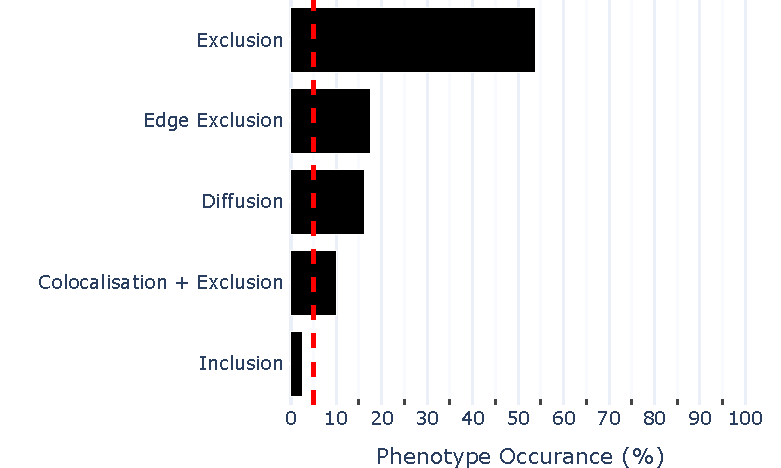
\includegraphics[width=1\linewidth]{08. Chapter 3/Figs/02. Infection/03. IFIT3/01. bar_i3_a549.pdf} 
    \end{subfigure}
    \begin{subfigure}{0.495\textwidth}
        \caption{}
        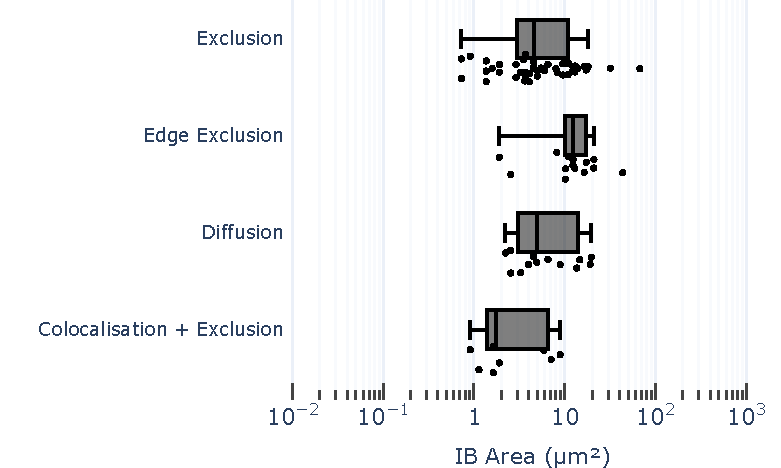
\includegraphics[width=1\linewidth]{08. Chapter 3/Figs/02. Infection/03. IFIT3/02. box_i3_a549.pdf}
    \end{subfigure}
    \caption[Phenotypic Diversity of hIFIT3 Interactions with hRSV Inclusion Bodies in A549 Cell Line.]{\textbf{Phenotypic Diversity of hIFIT3 Interactions with hRSV Inclusion Bodies in A549 Cell Line.} A549 cells were infected with human RSV at MOI 1 and fixed 24 HPI. Cells were double-labeled with with anti-RSV N and anti-IFIT3 antibodies and imaged on confocal microscope. Panel (a) shows percentual proportions of observed phenotypes between hRSV inclusion bodies and hIFIT3 (80 observations), with the red dotted line denoting the 5\% threshold, marking phenotypes considered relevant above this limit. Panel (b) shows the IB area in \(\mu \mbox{m}^2\) per observed relevant phenotype.}
    \label{fig:Phenotypic Diversity of hIFIT3 Interactions with hRSV Inclusion Bodies in A549 Cell Line}
\end{figure}

\begin{figure}
    \centering
    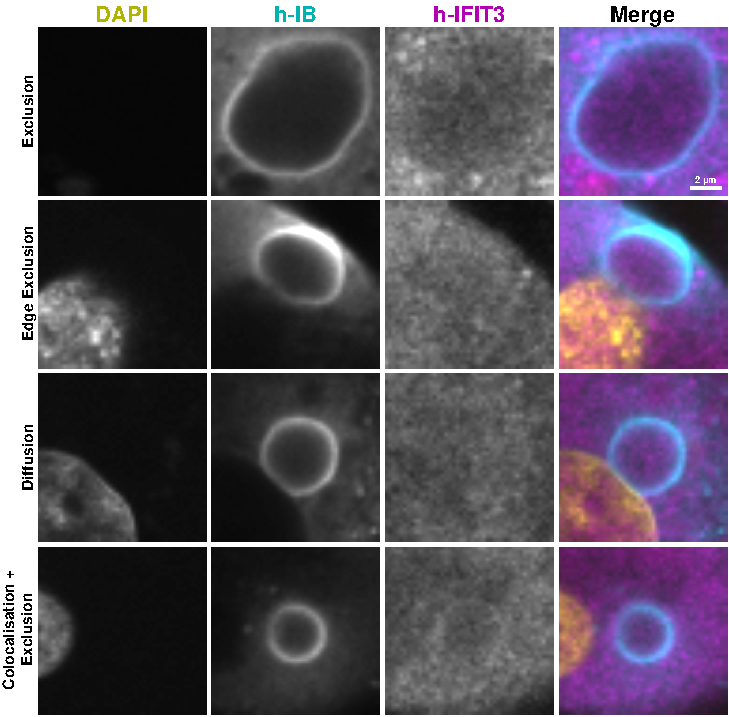
\includegraphics[width=1\linewidth]{08. Chapter 3/Figs/02. Infection/03. IFIT3/03. a549 i3.pdf}
    \caption[Representative Images of Phenotypic Diversity of hIFIT3 Interactions with hRSV Inclusion Bodies in A549 Cell Line.]{\textbf{Representative Images of Phenotypic Diversity of hIFIT3 Interactions with hRSV Inclusion Bodies in A549 Cell Line.} A549 cells were infected with hRSV at MOI 1 and fixed at 24 HPI. Cellular nuclei were stained with DAPI (yellow), and cells were double-labeled with anti-RSV N (cyan) and anti-IFIT3 (magenta) antibodies. This figure showcases representative examples of relevant phenotypes in the interaction between hIFIT3 and hRSV inclusion bodies. These phenotypes are presented in descending order based on their percentage proportions. The scale bar indicates 2 \(\mu \mbox{m}\).}
    \label{fig:Representative Images of Phenotypic Diversity of hIFIT3 Interactions with hRSV Inclusion Bodies in A549 Cell Line}
\end{figure}

To validate this data, we looked at the phenotypic diversity of interactions between human IFIT3 and hRSV IBs in the BEAS2B cell line. The observed phenotypes, along with the calculated occurrence frequencies and measured associated IB areas, are shown in Figure \ref{fig:Phenotypic Diversity of hIFIT3 Interactions with hRSV Inclusion Bodies in BEAS2B Cell Line}, with the representative images of these phenotypes being shown in Figure \ref{fig:Representative Images of Phenotypic Diversity of hIFIT3 Interactions with hRSV Inclusion Bodies in BEAS2B Cell Line}. It is to be noted that we acquired only a small amount of observations (16) from this cell line. Regardless, the obtained data mirrors observations from A549 in all aspects of the nature of observed phenotypes, the frequency of occurrence of these phenotypes, and the area of IBs associated with these phenotypes. In more detail, the most frequent phenotypic interaction was exclusion (62\% of observations), followed by diffusion (19\% of observations), edge exclusion (12\% of observations), and lastly colocalisation with the IB structure (6\% of observations). The typical size of IBs associated with the exclusion phenotype was 5.5 \(\mu \mbox{m}^2\), a value which is slightly higher than the median aggregate value for BEAS2B IBs (3 \(\mu \mbox{m}^2\)). The diffusion phenotype was detected predominantly from smaller IBs with a median area of 3 \(\mu \mbox{m}^2\), while the edge exclusion phenotype was observed in IBs with the typical size of 10 \(\mu \mbox{m}^2\). Lastly, we have observed one IB-IFIT3 interaction which resulted in colocalisation with the measured IB area of 2.3 \(\mu \mbox{m}^2\). It is remarkable that using such a small number of observations mirrors the results from the A549 cell line so well (as can be seen when compared to Figure \ref{fig:Phenotypic Diversity of hIFIT3 Interactions with hRSV Inclusion Bodies in A549 Cell Line}). Overall, this data validates the results obtained from the A549 cell line.

\begin{figure}
    \begin{subfigure}{0.495\textwidth}
        \caption{}
        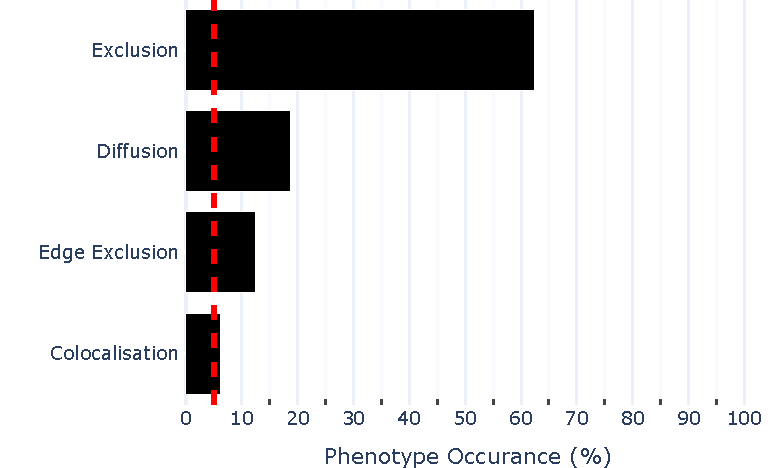
\includegraphics[width=1\linewidth]{08. Chapter 3/Figs/02. Infection/03. IFIT3/04. bar_i3_beas2b.pdf} 
    \end{subfigure}
    \begin{subfigure}{0.495\textwidth}
        \caption{}        
        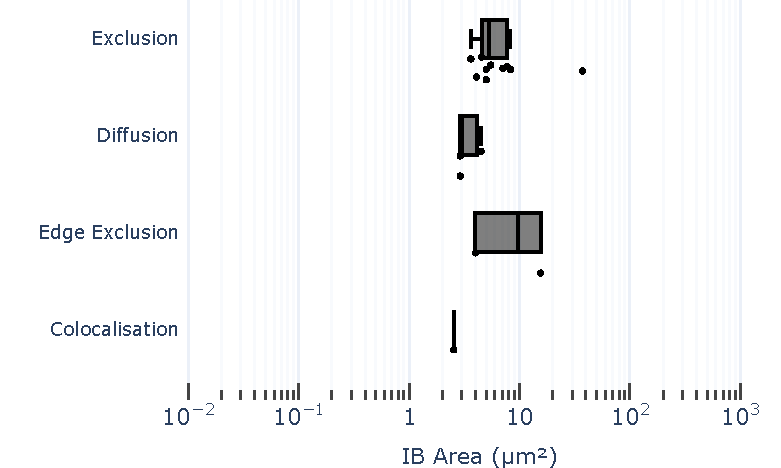
\includegraphics[width=1\linewidth]{08. Chapter 3/Figs/02. Infection/03. IFIT3/05. box_i3_beas2b.pdf}
    \end{subfigure}
    \caption[Phenotypic Diversity of hIFIT3 Interactions with hRSV Inclusion Bodies in BEAS2B Cell Line.]{\textbf{Phenotypic Diversity of hIFIT3 Interactions with hRSV Inclusion Bodies in BEAS2B Cell Line.} BEAS2B cells were infected with human RSV at MOI 1 and fixed 24 HPI. Cells were labeled with anti-RSV N and anti-IFIT3 antibodies and imaged on confocal microscope. Panel (a) shows percentual proportions of observed phenotypes between hRSV inclusion bodies and hIFIT3 (16 observations), with the red dotted line denoting the 5\% threshold, marking phenotypes considered relevant above this limit. Panel (b) shows the IB area in \(\mu \mbox{m}^2\) per observed relevant phenotype.}
    \label{fig:Phenotypic Diversity of hIFIT3 Interactions with hRSV Inclusion Bodies in BEAS2B Cell Line}
\end{figure}

\begin{figure}
    \centering
    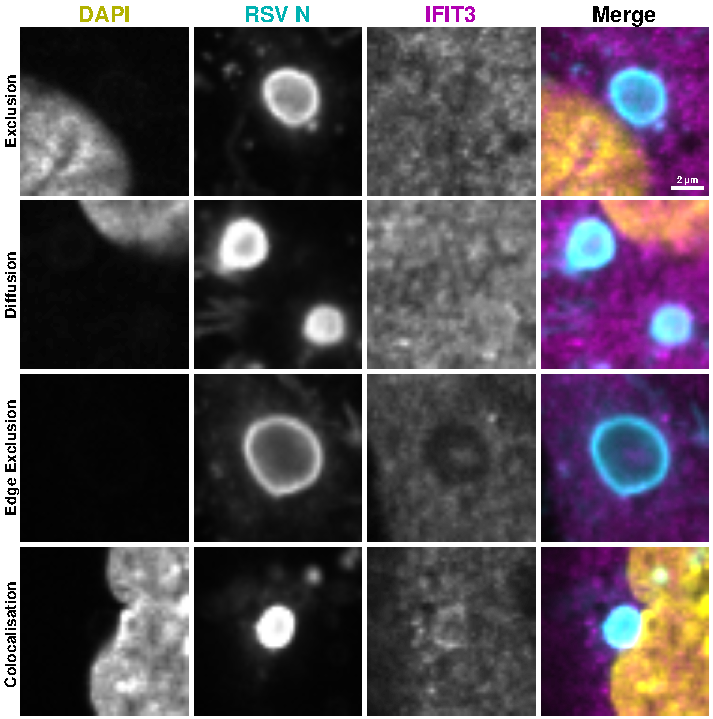
\includegraphics[width=1\linewidth]{08. Chapter 3/Figs/02. Infection/03. IFIT3/06. beas2b i3.pdf}
    \caption[Representative Images of Phenotypic Diversity of hIFIT3 Interactions with hRSV Inclusion Bodies in BEAS2B Cell Line]{\textbf{Representative Images of Phenotypic Diversity of hIFIT3 Interactions with hRSV Inclusion Bodies in BEAS2B Cell Line.} BEAS2B cells were infected with hRSV at MOI 1 and fixed at 24 HPI. Cellular nuclei were stained with DAPI (yellow), and cells were double-labelled with anti-RSV N (cyan) and anti-IFIT3 (magenta) antibodies. This figure showcases representative examples of relevant phenotypes in the interaction between hIFIT3 and hRSV inclusion bodies. These phenotypes are presented in descending order based on their percentage proportions. The scale bar indicates 2 \(\mu \mbox{m}\).}
    \label{fig:Representative Images of Phenotypic Diversity of hIFIT3 Interactions with hRSV Inclusion Bodies in BEAS2B Cell Line}
\end{figure}

Lastly, we set out to investigate the diversity of interactions between bovine IFIT3 and bRSV IBs in the MDBK cell line, as detected in 214 observations. Previous preliminary analysis suggested that bIFIT3 forms intra-IB inclusions that seem to possess substructures resembling IBAGs (Figure \ref{fig:Modulations in the Subcellular Localisation of Bovine IFITs in MDBK Cells Exposed to bIFNa or bRSV}). In the more detailed analysis, consisting of 214 observations, we observe the inclusion phenotype to be the second most prevalent interaction phenotype, confirming the previous results. The observed phenotypes, along with the calculated occurrence frequencies and measured associated IB areas, are shown in Figure \ref{fig:Phenotypic Diversity of bIFIT3 Interactions with bRSV Inclusion Bodies in MDBK Cell Line}, with the representative images of these phenotypes being shown in Figure \ref{fig:Representative Images of Phenotypic Diversity of bIFIT3 Interactions with bRSV Inclusion Bodies in MDBK Cell Line}. As observed in A549 and BEAS2B cell lines, the most prevalent interaction between bovine IFIT3 and IBs is exclusion from these structures, which occurs in 43\% of observations. The second most common phenotype is inclusion with 34\% frequency, followed up by diffusion and edge exclusion phenotypes, which occurred with 12\% and 9\% frequencies respectively. Lastly, we also observed inclusion cooccurring with intra-IB spots that resemble IBAGs, although only in 2\% of cases. With regards to the IB size profile categorised based on the different observed phenotypes, we can see that the exclusion, inclusion, and diffusion phenotypes display a similar range of values, ranging from sub 0.5 \(\mu \mbox{m}^2\) to supra 15 \(\mu \mbox{m}^2\), the distribution profile and especially the median values differ between them. While the typical values of exclusion and diffusion phenotype-associated IBs are shifted towards smaller IBs (1.2 \(\mu \mbox{m}^2\) and 1 \(\mu \mbox{m}^2\) respectively), the median size is 3.3 \(\mu \mbox{m}^2\), above the typical aggregate sizes detected in MDBK (2 \(\mu \mbox{m}^2\)). Lastly, the median size of IBs, from which bIFIT3 was observed to be edge excluded, was 11 \(\mu \mbox{m}^2\), encompassing mainly more mature IBs, larger than 3 \(\mu \mbox{m}^2\).

Taken together, consistent IFIT3/IB interaction patterns emerge, which appear to be species-independent. Similar to observations with IFIT1, IFIT3 is predominantly excluded from IB structures, irrespective of IB size. It is also frequently observed to be diffused throughout the entire IB structure, whether including or excluding the IB boundary. Due to the similarity of these two phenotypes in terms of the potential of IFIT3 interaction within IB structures, they could be treated with equal phenotypic significance. Interestingly, diffusion predominantly occurred in smaller IBs, while the edge exclusion phenotype was present in larger, more mature IBs. This suggests a potential link between these phenotypes, indicating a distribution shift dependent on IB maturation, gradually excluding IFIT3 from the periphery of the IB. Lastly, we observed direct IFIT3 interactions with IB structures in the form of inclusions or IB-boundary colocalisations, although these phenotypes were less prevalent. They occurred in both small and large IBs, suggesting that these interactions are not IB size-dependent.

\begin{figure}
    \begin{subfigure}{0.495\textwidth}
        \caption{}
        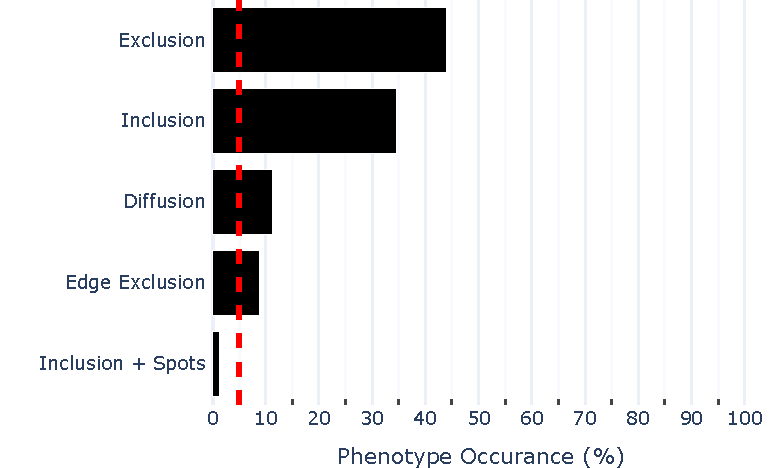
\includegraphics[width=1\linewidth]{08. Chapter 3/Figs/02. Infection/03. IFIT3/07. bar_i3_mdbk.pdf} 
    \end{subfigure}
    \begin{subfigure}{0.495\textwidth}
        \caption{}
        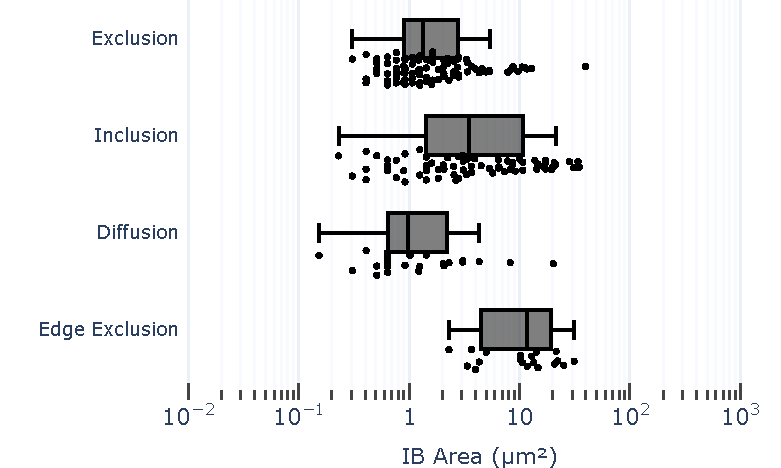
\includegraphics[width=1\linewidth]{08. Chapter 3/Figs/02. Infection/03. IFIT3/08. box_i3_mdbk.pdf}
    \end{subfigure}
    \caption[Phenotypic Diversity of bIFIT3 Interactions with bRSV Inclusion Bodies in MDBK Cell Line.]{\textbf{Phenotypic Diversity of bIFIT3 Interactions with bRSV Inclusion Bodies in MDBK Cell Line.} MDBK cells were infected with bovine RSV at MOI 1 and fixed 24 HPI. Cells were labelled with anti-RSV N and anti-IFIT3 antibodies and imaged on a confocal microscope. Panel (a) shows the percentual proportions of observed phenotypes between bRSV inclusion bodies and bIFIT3 (214 observations), with the red dotted line denoting the 5\% threshold, marking phenotypes considered relevant above this limit. Panel (b) shows the IB area in \(\mu \mbox{m}^2\) per observed relevant phenotype.}
    \label{fig:Phenotypic Diversity of bIFIT3 Interactions with bRSV Inclusion Bodies in MDBK Cell Line}
\end{figure}

\begin{figure}
    \centering
    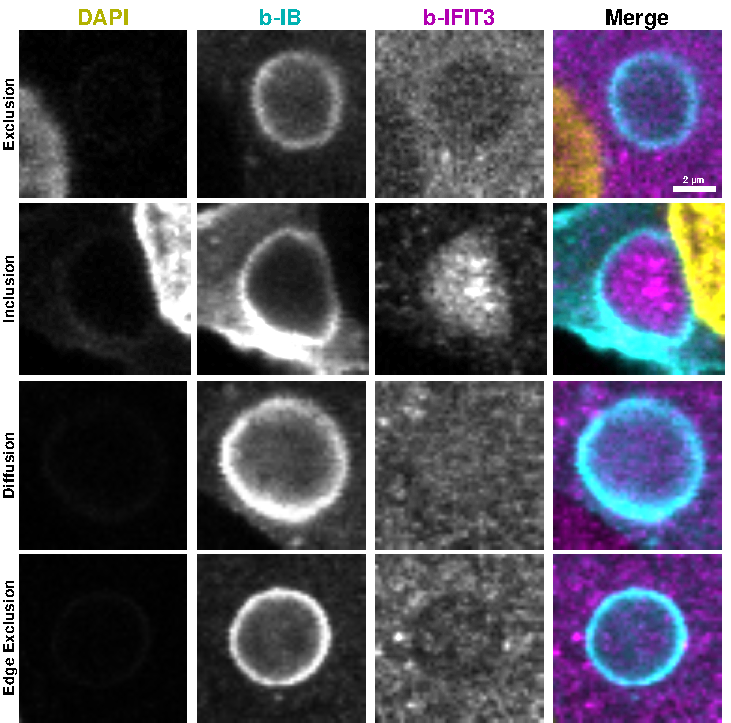
\includegraphics[width=1\linewidth]{08. Chapter 3/Figs/02. Infection/03. IFIT3/09. mdbk i3.pdf}
    \caption[Representative Images of Phenotypic Diversity of bIFIT3 Interactions with bRSV Inclusion Bodies in MDBK Cell Line.]{\textbf{Representative Images of Phenotypic Diversity of bIFIT3 Interactions with bRSV Inclusion Bodies in MDBK Cell Line.} MDBK cells were infected with bRSV at MOI 1 and fixed at 24 HPI. Cellular nuclei were stained with DAPI (yellow), and cells were double-labeled with anti-RSV N (cyan) and anti-IFIT3 (magenta) antibodies. This figure showcases representative examples of relevant phenotypes in the interaction between bIFIT3 and bRSV inclusion bodies. These phenotypes are presented in descending order based on their percentage proportions. The scale bar indicates 2 \(\mu \mbox{m}\).}
    \label{fig:Representative Images of Phenotypic Diversity of bIFIT3 Interactions with bRSV Inclusion Bodies in MDBK Cell Line}
\end{figure}

\subsubsection{Phenotypic Diversity of Endogenous IFIT5 Interaction with RSV IBs}
Lastly, we assayed the interactions of human and bovine IFIT5 protein with human and bovine RSV inclusion bodies. Initially, we investigated the diversity of interactions in the A549 cell line infected with hRSV at MOI 1 for 24 hours. We assayed 77 observations. Figure \ref{fig:Phenotypic Diversity of hIFIT5 Interactions with hRSV Inclusion Bodies in A549 Cell Line} shows the results of the analysis, while Figure \ref{fig:Representative Images of Phenotypic Diversity of hIFIT5 Interactions with hRSV Inclusion Bodies in A549 Cell Line} displays the representative images of interaction phenotypes with a frequency of occurrence of at least 5\%. We can see that 57\% of interactions result in the exclusion phenotype. This is followed by diffusion and edge exclusion phenotypes, occurring at the frequency of 17\% and 16\% respectively. These were followed by a colocalisation phenotype accompanied by exclusion, which occurred in 5\% of observations and was the last interaction phenotype that was included in the IB size analysis. We have, however, observed three more phenotypes, each occurring with only 1\% frequency. These were inclusion, edge exclusion accompanied by the presence of spots, and colocalisation phenotypes. With regards to the size profile of IBs associated with the phenotypic interaction that occurred with higher than 5\% frequency, exclusion-associated IBs show a distribution similar to the aggregate distribution of all detected IBs in A549 cell line, ranging from sub 1 \(\mu \mbox{m}^2\) to supra 30 \(\mu \mbox{m}^2\) measured areas, with the median value of 6.3 \(\mu \mbox{m}^2\). We can hence assume that this phenotype happens in the whole population of IBs, regardless of the state of maturity. The IBs associated with the diffusion phenotype had a median size value of 4 \(\mu \mbox{m}^2\) and were restricted in their maximal size (<10 \(\mu \mbox{m}^2\)). The last two phenotypes, edge exclusion and colocalisation accompanied by exclusion, both happened in IBs with sizes larger than 3 \(\mu \mbox{m}^2\), suggesting a certain level of IB maturity was necessary for these phenotypes to occur. In more detail, edge exclusion occurred in IBs with the median size of 8 \(\mu \mbox{m}^2\), while the latter had a typical size of 13 \(\mu \mbox{m}^2\).

\begin{figure}
    \begin{subfigure}{0.495\textwidth}
        \caption{}
        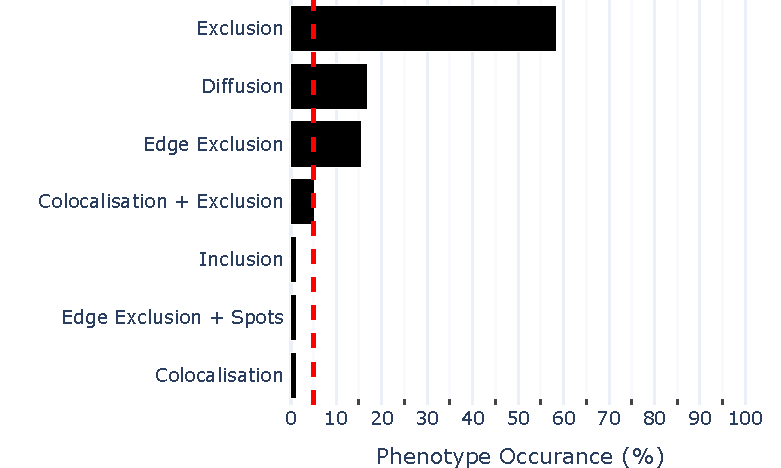
\includegraphics[width=1\linewidth]{08. Chapter 3/Figs/02. Infection/04. IFIT5/01. bar_i5_a549.pdf} 
    \end{subfigure}
    \begin{subfigure}{0.495\textwidth}
        \caption{}
        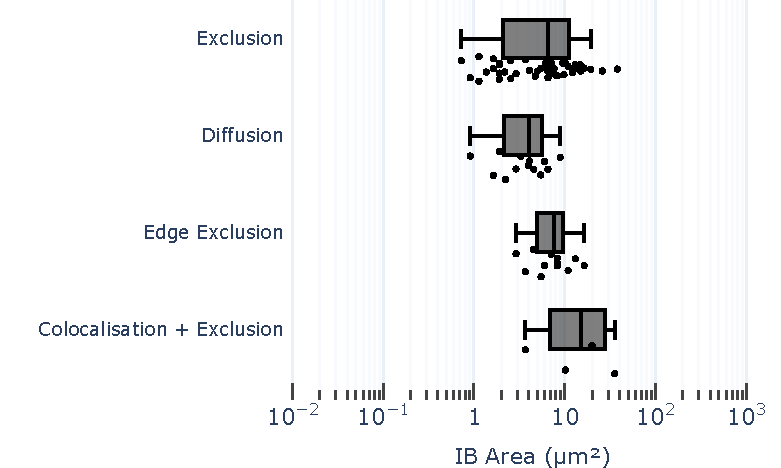
\includegraphics[width=1\linewidth]{08. Chapter 3/Figs/02. Infection/04. IFIT5/02. box_i5_a549.pdf}
    \end{subfigure}
    \caption[Phenotypic Diversity of hIFIT5 Interactions with hRSV Inclusion Bodies in A549 Cell Line.]{\textbf{Phenotypic Diversity of hIFIT5 Interactions with hRSV Inclusion Bodies in A549 Cell Line.} A549 cells were infected with human RSV at MOI 1 and fixed 24 HPI. Cells were labelled with anti-RSV N and anti-IFIT5 antibodies and imaged on a confocal microscope. Panel (a) shows the percentual proportions of observed phenotypes between hRSV inclusion bodies and hIFIT5 (77 observations), with the red dotted line denoting the 5\% threshold, marking phenotypes considered relevant above this limit. Panel (b) shows the IB area in \(\mu \mbox{m}^2\) per observed relevant phenotype.}
    \label{fig:Phenotypic Diversity of hIFIT5 Interactions with hRSV Inclusion Bodies in A549 Cell Line}
\end{figure}

\begin{figure}
    \centering
    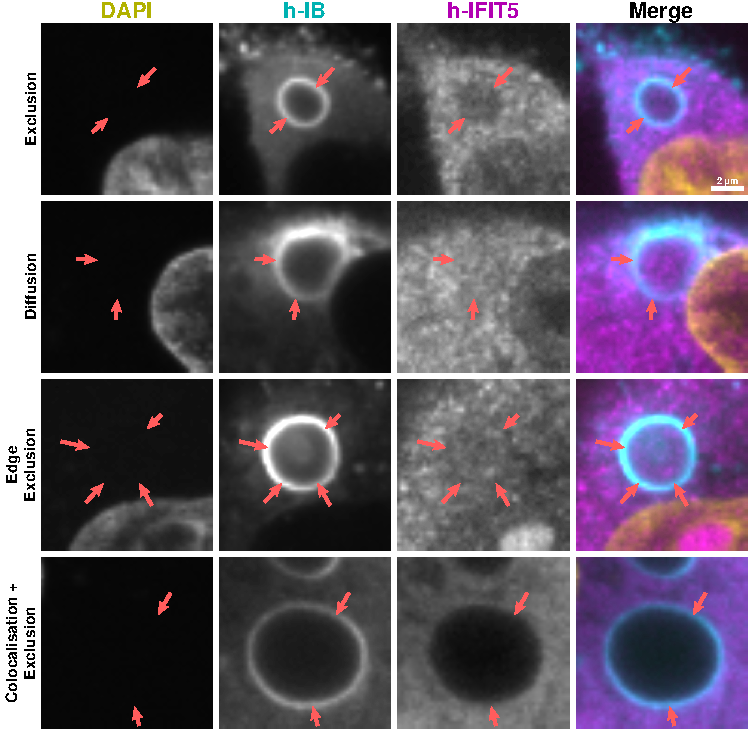
\includegraphics[width=1\linewidth]{08. Chapter 3/Figs/02. Infection/04. IFIT5/03. a549 i5.pdf}
    \caption[Representative Images of Phenotypic Diversity of hIFIT5 Interactions with hRSV Inclusion Bodies in A549 Cell Line.]{\textbf{Representative Images of Phenotypic Diversity of hIFIT5 Interactions with hRSV Inclusion Bodies in A549 Cell Line.} A549 cells were infected with hRSV at MOI 1 and fixed at 24 HPI. Cellular nuclei were stained with DAPI (yellow), and cells were double-labeled with anti-RSV N (cyan) and anti-IFIT5 (magenta) antibodies. This figure showcases representative examples of relevant phenotypes in the interaction between hIFIT5 and hRSV inclusion bodies. These phenotypes are presented in descending order based on their percentage proportions. The scale bar indicates 2 \(\mu \mbox{m}\).}
    \label{fig:Representative Images of Phenotypic Diversity of hIFIT5 Interactions with hRSV Inclusion Bodies in A549 Cell Line}
\end{figure}

We followed this with a validation of these findings in the BEAS2B cell line infected with hRSV. Figure \ref{fig:Phenotypic Diversity of hIFIT5 Interactions with hRSV Inclusion Bodies in BEAS2B Cell Line} shows the results of the analysis, while Figure \ref{fig:Representative Images of Phenotypic Diversity of hIFIT5 Interactions with hRSV Inclusion Bodies in BEAS2B Cell Line} displays the representative images of the observed interactions. Although only assessing 21 observations, we see similar results to what we observed in the A549 cell line. 62\% of IFIT5-hRSV IB observations seem to be excluded from these structures. This is followed by diffusion and edge exclusion phenotypes, both of which appear in 18\% of cases. In terms of the associated IB size profile, all three phenotype median sizes were similar (1.8 \(\mu \mbox{m}^2\), 2.3 \(\mu \mbox{m}^2\), and 3 \(\mu \mbox{m}^2\) respectively), although the exclusion phenotype encompasses the largest range of IB sizes (from sub 0.8 \(\mu \mbox{m}^2\) to 10 \(\mu \mbox{m}^2\)). The diffusion-associated IBs clustered in two size ranges, of around 1 \(\mu \mbox{m}^2\) and 4 \(\mu \mbox{m}^2\), while the edge exclusion-associated IBs tended to cluster more closely to their median value and did not occur in IBs with extremely small or large values. Overall, although we had a limited amount of observation, this data shows identical results to 92\% of observations from the A549 cell line.

\begin{figure}
    \begin{subfigure}{0.495\textwidth}
        \caption{}
        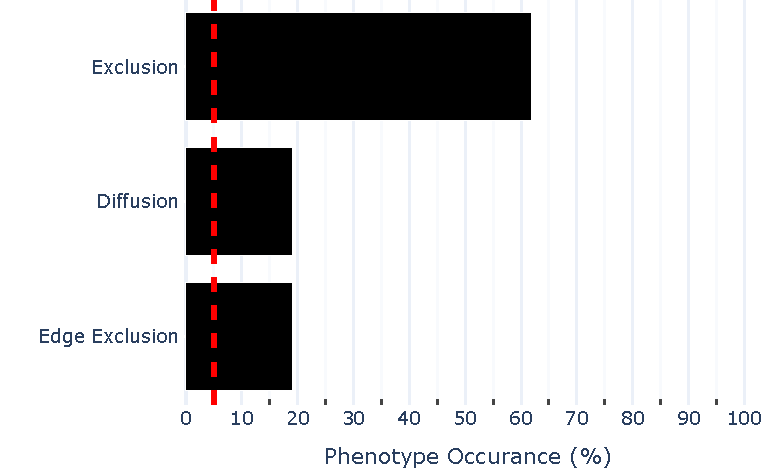
\includegraphics[width=1\linewidth]{08. Chapter 3/Figs/02. Infection/04. IFIT5/04. bar_i5_beas2b.pdf}
    \end{subfigure}
    \begin{subfigure}{0.495\textwidth}
        \caption{}
        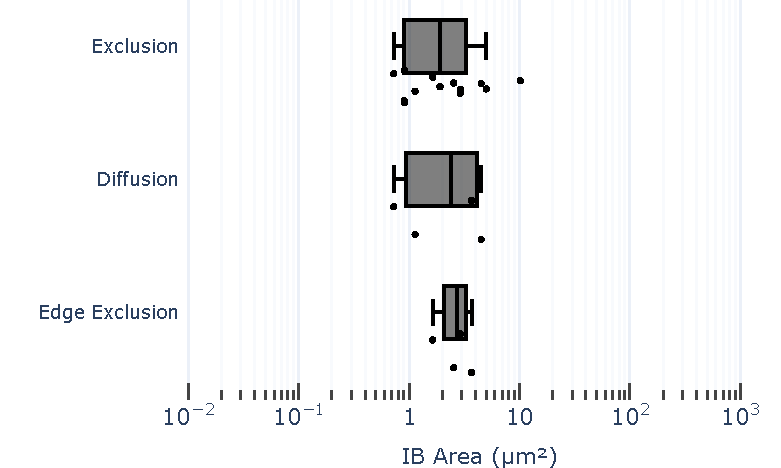
\includegraphics[width=1\linewidth]{08. Chapter 3/Figs/02. Infection/04. IFIT5/05. box_i5_beas2b.pdf}
    \end{subfigure}
    \caption[Phenotypic Diversity of hIFIT5 Interactions with hRSV Inclusion Bodies in BEAS2B Cell Line.]{\textbf{Phenotypic Diversity of hIFIT5 Interactions with hRSV Inclusion Bodies in BEAS2B Cell Line.} BEAS2B cells were infected with human RSV at MOI 1 and fixed 24 HPI. Cells were labelled with anti-RSV N and anti-IFIT5 antibodies and imaged on a confocal microscope. Panel (a) shows the percentual proportions of observed phenotypes between hRSV inclusion bodies and hIFIT5 (21 observations), with the red dotted line denoting the 5\% threshold, marking phenotypes considered relevant above this limit. Panel (b) shows the IB area in \(\mu \mbox{m}^2\) per observed relevant phenotype.}
    \label{fig:Phenotypic Diversity of hIFIT5 Interactions with hRSV Inclusion Bodies in BEAS2B Cell Line}
\end{figure}

\begin{figure}
    \centering
    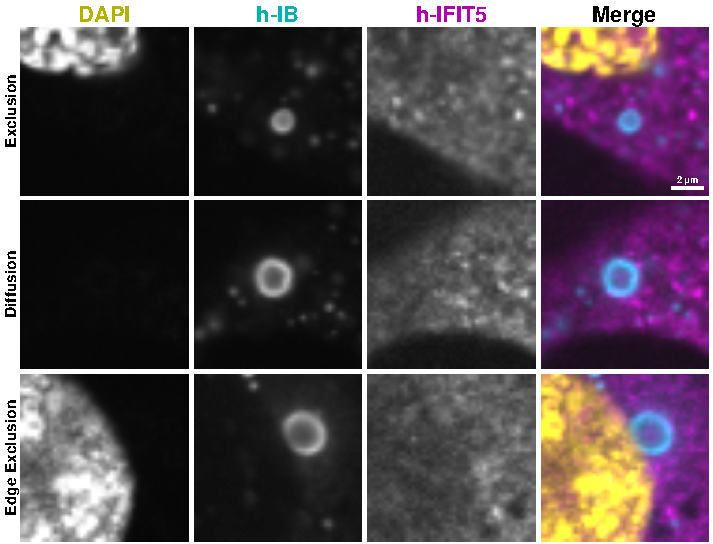
\includegraphics[width=1\linewidth]{08. Chapter 3/Figs/02. Infection/04. IFIT5/06. beas2b i5.pdf}
    \caption[Representative Images of Phenotypic Diversity of hIFIT5 Interactions with hRSV Inclusion Bodies in BEAS2B Cell Line.]{\textbf{Representative Images of Phenotypic Diversity of hIFIT5 Interactions with hRSV Inclusion Bodies in BEAS2B Cell Line.} BEAS2B cells were infected with hRSV at MOI 1 and fixed at 24 HPI. Cellular nuclei were stained with DAPI (yellow), and cells were double-labeled with anti-RSV N (cyan) and anti-IFIT5 (magenta) antibodies. This figure showcases representative examples of relevant phenotypes in the interaction between hIFIT5 and hRSV inclusion bodies. These phenotypes are presented in descending order based on their percentage proportions. The scale bar indicates 2 \(\mu \mbox{m}\).}
    \label{fig:Representative Images of Phenotypic Diversity of hIFIT5 Interactions with hRSV Inclusion Bodies in BEAS2B Cell Line}
\end{figure}

Lastly, we investigated the phenotypes of interactions of bovine IFIT5 with bRSV IBs in the MDBK cell line. The percentage frequencies of the 61 observations, along with the IB size analysis of the phenotypes occurring more often than 5\%, are shown in Figure \ref{fig:Phenotypic Diversity of bIFIT5 Interactions with bRSV Inclusion Bodies in MDBK Cell Line}, with the representative images of the latter shown in Figure \ref{fig:Representative Images of Phenotypic Diversity of bIFIT5 Interactions with bRSV Inclusion Bodies in MDBK Cell Line}. As observed in the human cell lines, the exclusion phenotype is the most common (51\% of observations), with the sizes of its associated IBs ranging from sub 0.5 \(\mu \mbox{m}^2\) to supra 20 \(\mu \mbox{m}^2\), although their distribution was skewed towards sub 3 \(\mu \mbox{m}^2\), with the median area of 1 \(\mu \mbox{m}^2\). This is below the typical value of aggregate MDBK IB observations, which had a median size of 2 \(\mu \mbox{m}^2\). Next, edge exclusion, which occurred in 29\% of cases, was observed predominantly in large, more mature IBs. Although some smaller IBs were observed with this phenotype as well, in general, they clustered in line with their typical size value of 13 \(\mu \mbox{m}^2\). Contrary to what we observed in the human cell lines previously, the inclusion phenotype occurs in 10\% of observations. Inclusion-associated IBs tend to be smaller in size with the median value of 3 \(\mu \mbox{m}^2\), with all of these being smaller than 4 \(\mu \mbox{m}^2\) (with the exception of one observation which was 9.5 \(\mu \mbox{m}^2\) in size). Last to be observed phenotypes were diffusion, and edge exclusion co-observed with spots, which occurred at 8\% and 2\% respectively. The latter was not included in the size analysis as it did not occur with a frequency higher than 5\%. For the former, the observed IB sizes associated with this phenotype had a typical size of 0.9 \(\mu \mbox{m}^2\).

In summary, across all cell lines, the exclusion phenotype dominates IFIT5/IB interactions, constituting more than 50\% of observed interactions. This prevalent interaction occurs in IBs of varying sizes, from sub 1 \(\mu \mbox{m}^2\) to supra \(\mu \mbox{m}^2\), suggesting no specific association with a distinct IB population. The two other consistently common phenotypes are IB edge exclusion and diffusion. The resemblance in the distribution of these phenotypes suggests a potential relationship, possibly representing distinct phases of the same interaction phenotype. This is supported by the observation that the diffusion phenotype occurs in small and medium-sized IBs, while the edge exclusion phenotype is prevalent in medium and large-sized IBs. This suggests a scenario in which IFIT5 diffuses through a population of small, immature IBs, progressively relocating from the IB boundary as the IBs enlarge and lose their liquid-like nature. Finally, we noted less frequent direct interaction phenotypes, namely colocalisation/exclusion and intra-IB inclusion, observed in A549 and MDBK cell lines. The lower overall frequency could explain why they were not detected in the BEAS2B cell line, as the total number of observations in this cell line was fewer. Collectively, these findings suggest a conserved propensity for IFIT5 to interact with RSV IB structures across species.

\begin{figure}
    \begin{subfigure}{0.495\textwidth}
        \caption{}
        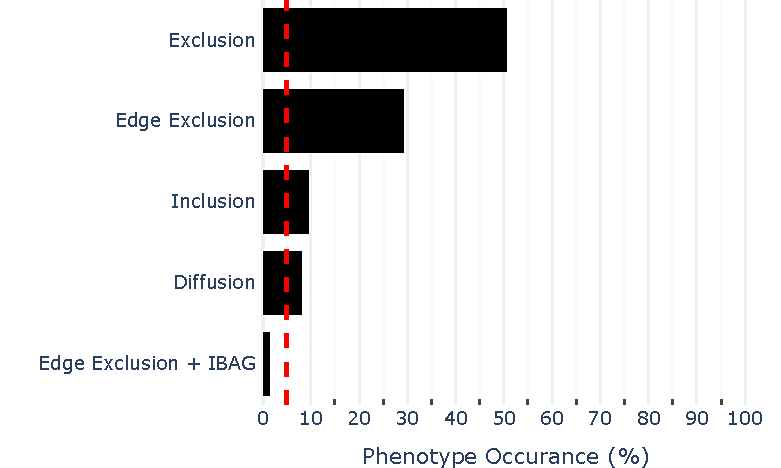
\includegraphics[width=1\linewidth]{08. Chapter 3/Figs/02. Infection/04. IFIT5/07. bar_i5_mdbk.pdf} 
    \end{subfigure}
    \begin{subfigure}{0.495\textwidth}
        \caption{}
        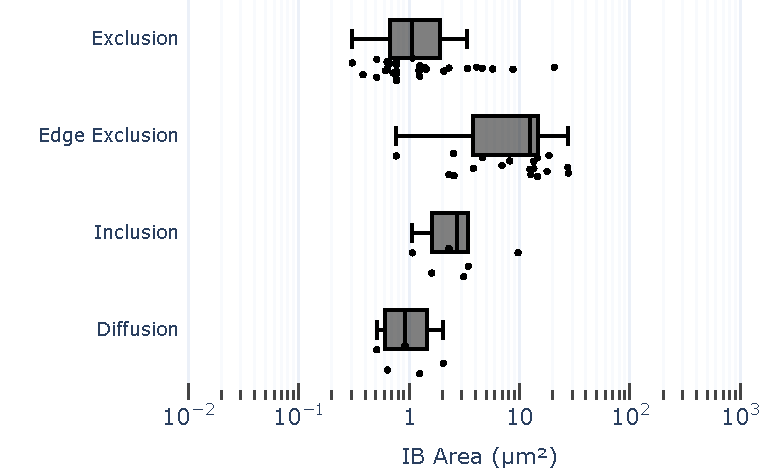
\includegraphics[width=1\linewidth]{08. Chapter 3/Figs/02. Infection/04. IFIT5/08. box_i5_mdbk.pdf}
    \end{subfigure}
    \caption[Phenotypic Diversity of bIFIT5 Interactions with bRSV Inclusion Bodies in MDBK Cell Line.]{\textbf{Phenotypic Diversity of bIFIT5 Interactions with bRSV Inclusion Bodies in MDBK Cell Line.} MDBK cells were infected with bovine RSV at MOI 1 and fixed 24 HPI. Cells were labelled with anti-RSV N and anti-IFIT5 antibodies and imaged on a confocal microscope. Panel (a) shows the percentual proportions of observed phenotypes between bRSV inclusion bodies and bIFIT5 (61 observations), with the red dotted line denoting the 5\% threshold, marking phenotypes considered relevant above this limit. Panel (b) shows the IB area in \(\mu \mbox{m}^2\) per observed relevant phenotype.}
    \label{fig:Phenotypic Diversity of bIFIT5 Interactions with bRSV Inclusion Bodies in MDBK Cell Line}
\end{figure}

\begin{figure}
    \centering
    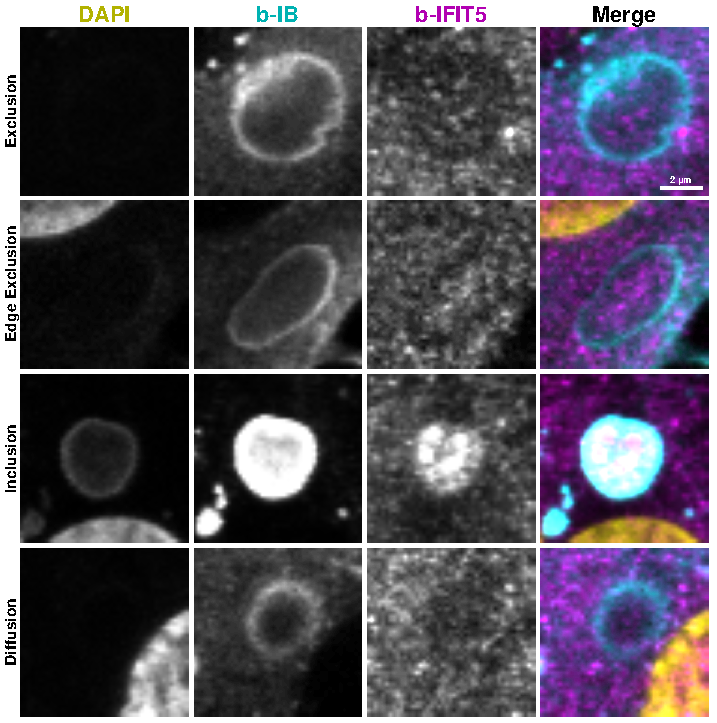
\includegraphics[width=1\linewidth]{08. Chapter 3/Figs/02. Infection/04. IFIT5/09. mdbk i5.pdf}
    \caption[Representative Images of Phenotypic Diversity of bIFIT5 Interactions with bRSV Inclusion Bodies in MDBK Cell Line.]{\textbf{Representative Images of Phenotypic Diversity of bIFIT5 Interactions with bRSV Inclusion Bodies in MDBK Cell Line.} MDBK cells were infected with bRSV at MOI 1 and fixed at 24 HPI. Cellular nuclei were stained with DAPI (yellow), and cells were double-labeled with anti-RSV N (cyan) and anti-IFIT5 (magenta) antibodies. This figure showcases representative examples of relevant phenotypes in the interaction between bIFIT5 and bRSV inclusion bodies. These phenotypes are presented in descending order based on their percentage proportions. The scale bar indicates 2 \(\mu \mbox{m}\).}
    \label{fig:Representative Images of Phenotypic Diversity of bIFIT5 Interactions with bRSV Inclusion Bodies in MDBK Cell Line}
\end{figure}